%%%%%%%%%%%%%%%%%%%%%%%%%%%%%%%%%%%%%%%%%%%%%%%%%
%%                                             %%
%%    Grounding the Interaction: Knowledge     %%
%%      Management for Interactive Robots      %%
%%                                             %%
%%               PhD Thesis                    %%
%%                                             %%
%%%%%%%%%%%%%%%%%%%%%%%%%%%%%%%%%%%%%%%%%%%%%%%%%

%% Author:     Séverin Lemaignan


\documentclass[a4paper,12pt]{book}

\usepackage{fullpage}

\usepackage{appendix}

\usepackage{graphicx}
\usepackage{xstring}
\usepackage[footnotesize,margin=1cm]{caption}

\usepackage[table]{xcolor}

\usepackage{ifthen}

\usepackage[utf8]{inputenc}

\usepackage[T1]{fontenc}
\pdfmapfile{+ubuntu-regular.map}
\pdfmapfile{+ubuntu-it.map}
\pdfmapfile{+ubuntu-bold.map}
\renewcommand{\rmdefault}{Ubuntu}

\usepackage{listings}
\usepackage{alltt}
\usepackage{pseudocode}
\usepackage{fancyvrb}

%diagrams
\usepackage{tikz}
\usetikzlibrary{shapes}

\usepackage{wrapfig}
\usepackage{subfigure}
\usepackage{fancyhdr} %headers and footers
\pagestyle{fancy}

%tables
\usepackage{booktabs}
\usepackage{tabularx}
\usepackage{multirow}
\usepackage{varwidth}
\newcommand{\turn}[3][10em]{% \turn[<width>]{<angle>}{<stuff>}
  \rlap{\rotatebox{#2}{\begin{varwidth}[t]{#1}\bfseries#3\end{varwidth}}}%
  }
\usepackage{pdflscape} %% Used for very big table

\usepackage{url}
\usepackage{hyperref}
\usepackage{sectsty}

\usepackage{enumerate}
\usepackage{paralist}

\usepackage{pdfpages} %% To add a cover to the doc

% Fixme notes
\usepackage[draft,footnote,marginclue]{fixme}

\usepackage[toc]{glossaries}

\usepackage[english]{babel}

%%%%%%%%%%%%%%%%%%%%%%%%%%%%%%%%%%%%%%%%%%%%%%%%%%%%%%%%%%%%%%%%%%%%%%%%%%%%%%%
%%%%%%%%%%%%%%%%%%%%%%%%%%%%%%%%%%%%%%%%%%%%%%%%%%%%%%%%%%%%%%%%%%%%%%%%%%%%%%%
%%                        MACROS and glossary


%%%%%%%%%%%%%%%%%%%%%%%%%%%%%%%%%%%%%%%%%%%%%%%%%%%%%%%%%%%%%%%%%%%%%%%%%%%%%%%
%%                           Glossary                                        %%
%%%%%%%%%%%%%%%%%%%%%%%%%%%%%%%%%%%%%%%%%%%%%%%%%%%%%%%%%%%%%%%%%%%%%%%%%%%%%%%
\makeglossaries
%Pour re-générer le glossaire : makeindex these.glo -s these.ist -t these.glg -o these.gls
%\newglossaryentry{parametre}
%		{name={paramètre}, 
%		description={Un paramètre d'une fonction est une option que l'on passe à la fonction et que l'on peut modifier.}}
%%%%%%%%%%%%%%%%%%%%%%%%%%%%%%%%%%%%%%%%%%%%%%%%%%%%%%%%%%%%%%%%%%%%%%%%%%%%%%%

\newcommand{\meth}[3]{\texttt{#1 {\bf #2}(#3)}}

%Name of the speaker in a chat
\newcommand{\chatN}[1]{{\footnotesize \textsf{#1}}}
\newcommand{\concept}[1]{{\small \texttt{#1}}}

%\newcommand{\stmt}[1]{{\footnotesize \tt $\langle$ #1\relax$\rangle$}}
\newcommand{\stmt}[1]{{\footnotesize $\langle\stmttt#1\relax\rangle$}}
\newcommand{\rawstmt}[1]{{\footnotesize \stmttt#1\relax}}
\def\stmttt#1 #2 #3\relax{
\texttt{\IfBeginWith{#1}{?}{\textbf{#1}}{#1} \IfBeginWith{#2}{?}{\textbf{#2}}{\emph{#2}} \ifthenelse {\equal{#3}{true} \OR \equal{#3}{false}}{\emph{#3}}{\IfBeginWith{#3}{?}{\textbf{#3}} {#3}}}}

\newcommand{\setstmt}[1]{{\footnotesize [\setstmttt#1\relax]}}
\def\setstmttt#1,#2\relax{\stmttt#1\relax, \stmttt#2\relax}

% Java class/interface
\newcommand{\jmeth}[1]{{\texttt{#1}}}
\newcommand{\jclass}[1]{{\texttt{#1}}}
\newcommand{\jinterface}[1]{{\texttt{#1}}}

\newcommand{\ie}{{\textit{i.e.\ }}}
\newcommand{\cf}{{\textit{cf\ }}}
\newcommand{\eg}{{\textit{e.g.\ }}}

%Met par defaut la taille en scriptsize et la font en sans serif pour les notes dans la marge
\let\myMargin\marginpar
\renewcommand{\marginpar}[1]{\myMargin{{\scriptsize \sffamily #1}}}

\graphicspath{{images/}}

%%%%%%%%%%%%%%%%%%%%%%%%%%%%%%%%%%%%%%%%%%%%%%%%%%%%%%%%%%%%%%%%%%%%%%%%%%%%%%%%%%%%%%%%%%%%%%%%%%%%%%%
%%%%%%%%%%%%%%%%%%%%%%%%%%%%%%%%%%%%%%%%%%%%%%%%%%%%%%%%%%%%%%%%%%%%%%%%%%%%%%%%%%%%%%%%%%%%%%%%%%%%%%%
%%                                   LAYOUT (with fancyhdr)

\headheight=14.85pt
%pour récupérer les noms de section en minuscule
\renewcommand{\chaptermark}[1]{\markboth{#1}{}}
\renewcommand{\sectionmark}[1]{\markright{#1}}

% Redefine plain page style (for special case like 'chapter' that automatically goes back to it.
\fancypagestyle{plain}{\fancyhead{}\renewcommand{\headrulewidth}{0pt}}

% Define base pagestyle
\fancyhf{}
% Headers
\fancyhead[RO, LE]{\bfseries\leftmark}
%\fancyhead[LE]{\rightmark}
\renewcommand{\headrulewidth}{0.3pt}
\addtolength{\headheight}{2pt}
\addtolength{\headsep}{20pt}

% Footers
\fancyfoot[LE,RO]{\bfseries\thepage}
\addtolength{\footskip}{10pt}
\renewcommand{\footrulewidth}{0pt}


% Code for creating empty pages
% No headers on empty pages before new chapter
\makeatletter
\def\cleardoublepage{\clearpage\if@twoside \ifodd\c@page\else
    \hbox{}
    \thispagestyle{plain}
    \newpage
    \if@twocolumn\hbox{}\newpage\fi\fi\fi}
\makeatother \clearpage{\pagestyle{plain}\cleardoublepage}


%%%%%%%%%%%%%%%%%%%%%%%%%%%%%%%%%%%%%%%%%%%%%%%%%%%%%%%%%%%%%%%%%%%%%%%%%%%%%%%%%%%%%%%%%%%%%%%%%%%%%%%
%%%%%%%%%%%%%%%%%%%%%%%%%%%%%%%%%%%%%%%%%%%%%%%%%%%%%%%%%%%%%%%%%%%%%%%%%%%%%%%%%%%%%%%%%%%%%%%%%%%%%%%
%%       Listings general layout

\definecolor{dkgreen}{rgb}{0,0.6,0}
\definecolor{gray}{rgb}{0.5,0.5,0.5}
\definecolor{mauve}{rgb}{0.58,0,0.82}

\definecolor{molo-identifier}{HTML}{FD971F}
\definecolor{molo-string}{HTML}{229911}
\definecolor{molo-comment}{HTML}{75715E}

\lstset{basicstyle=\small, 
        captionpos=b, 
        frame=single,
        %backgroundcolor=\color{black},
        keywordstyle=\color{molo-identifier}\bf,          % keyword style
        commentstyle=\color{molo-comment},       % comment style
        stringstyle=\color{molo-string},         % string literal style
}

%%%%%%%%%%%%%%%%%%%%%%%%%%%%%%%%%%%%%%%%%%%%%%%%%%%%%%%%%%%%%%%%%%%%%%%%%%%%%%%%%%%%%%%%%%%%%%%%%%%%%%%
%%%%%%%%%%%%%%%%%%%%%%%%%%%%%%%%%%%%%%%%%%%%%%%%%%%%%%%%%%%%%%%%%%%%%%%%%%%%%%%%%%%%%%%%%%%%%%%%%%%%%%%
\title{
    \vspace{3em}
    \LARGE{\textbf{Grounding the Interaction: Knowledge Management for
    Interactive Robots}}\\[1cm]
    %\large{...}\\[1cm]
    \vfill
}

\author{
Séverin Lemaignan
}

%%%%%%%%%%%%%%%%%%%%%%%%%%%%%%%%%%%%%%%%%%%%%%%%%%%%%%%%%%%%%%%%%%%%%%%%%%%%%%%%%%%%%%%%%%%%%%%%%%%%%%%
%%%%%%%%%%%%%%%%%%%%%%%%%%%%%%%%%%%%%%%%%%%%%%%%%%%%%%%%%%%%%%%%%%%%%%%%%%%%%%%%%%%%%%%%%%%%%%%%%%%%%%%
\begin{document}

\tikzstyle {taxonomy} = [grow=right, level distance = 3cm, sibling distance=7mm]
\tikzstyle {completetaxonomy} = [grow=right]
\tikzstyle {taxon} = [text width=3cm, text centered,inner sep=0pt, outer sep=2pt] %, draw=blue!50,thick]


\IfFileExists{cover.pdf}{
\includepdf[pages=-, fitpaper]{cover.pdf}
\thispagestyle{empty}
\cleardoublepage
}

\maketitle

%%%%%%%%%%%%%%%%%%%%%%%%%%%%%%%%%%%%%%%%%%%%%%%%%%%%%%%%%%%%%%%%%%%%%%%%%%%%%%%%%%%%%%%%%%%%%%%%%%%%%%%
%%%%%%%%%%%%%%%%%%%%%%%%%%%%%%%%%%%%%%%%%%%%%%%%%%%%%%%%%%%%%%%%%%%%%%%%%%%%%%%%%%%%%%%%%%%%%%%%%%%%%%%

\frontmatter

\setcounter{tocdepth}{2}
\tableofcontents

\clearpage
\listoffixmes


\chapter*{\centering \begin{normalsize}Thanks\end{normalsize}}
\begin{quotation}
\noindent % abstract text
Thanks to...
\end{quotation}
\clearpage

\addcontentsline{toc}{chapter}{Abstract}
\chapter*{\centering \begin{normalsize}Abstract\end{normalsize}}
\begin{quotation}
\noindent % abstract text

With the rise of the so-called \emph{cognitive robotics}, the need of advanced
tools to store, manipulate, reason about the knowledge acquired by the robot
has been made clear. But storing and manipulating knowledge requires first to
understand what the knowledge \emph{itself} means to the robot and how to
represent it in a machine-processable way.

This work strives first at providing a systematic study of the knowledge
requirements of modern robotic applications in the context of service robotics
and human-robot interaction. What are the expressiveness requirement for a
robot? what are its needs in term of reasoning techniques? what are the
requirement on the robot's knowledge processing structure induced by other
cognitive functions like perception or decision making? We propose a novel
typology of desirable features for \emph{knowledge representation systems}
supported by an extensive review of existing tools in our community.

In a second part, the thesis presents in depth a particular instanciation of a
knowledge representation and manipulation system called \emph{ORO}, that has
been designed and implemented during the preparation of the thesis. We
elaborate on the inner working of this system, as well as its integration into
several complete robot control stacks. A particular focus is given to the
modelisation of agent-dependent symbolic perspectives and their relations to
theories of mind.

The third part of the study is focused on the presentation of one important
application of knowledge representation systems in the human-robot interaction
context: natural language understanding. Our approach and associated algorithms
leading to the grounding of unconstraint verbal interactions are presented,
followed by several experiments that have taken place both at the {\it
Laboratoire d'Analyse et d'Architecture des Systèmes} at CNRS, Toulouse and at
the {\it Intelligent Autonomous System} group at Munich Technical University.

The thesis concludes on considerations regarding the viability and importance
of an explicit management of the agent's knowledge, along with a reflexion on
the missing bricks in our research community on the way towards \emph{``human
level robots''}.

\end{quotation}
\clearpage

\addcontentsline{toc}{chapter}{Résumé}
\chapter*{\centering \begin{normalsize}Résumé\end{normalsize}}
\begin{quotation}
\noindent {\bf Ancrer l'interaction: Gestion des connaissances pour la robotique interactive}


\vspace{2em}

Avec le développement de la \emph{robotique cognitive}, le besoin d'outils
avancés pour représenter, manipuler, raisonner sur les connaissances acquises
par un robot a clairement été mis en avant. Mais stocker et manipuler des
connaissances requiert tout d'abord d'éclaircir ce que l'on nomme
\emph{connaissance} pour un robot, et comment celle-ci peut-elle être
représentée de manière intelligible pour une machine.

Ce travail s'efforce dans un premier temps d'identifier de manière systématique
les besoins en terme de représentation de connaissance des applications
robotiques modernes, dans le contexte spécifique de la robotique de service et
des interactions homme-robot. Nous proposons une typologie originale des
caractéristiques souhaitables des systèmes de représentation des connaissances,
appuyée sur un état de l'art détaillé des outils existants dans notre
communauté.

Dans un second temps, nous présentons en profondeur ORO, une instanciation
particulière d'un système de représentation et manipulation des connaissances,
conçu et implémenté durant la préparation de cette thèse. Nous détaillons le
fonctionnement interne du système, ainsi que son intégration dans plusieurs
architectures robotiques complètes. Un éclairage particulier est donné sur la
modélisation de la prise de perspective dans le contexte de l'interaction, et de
son interprétation en terme de théorie de l'esprit.

La troisième partie de l'étude porte sur une application importante des
systèmes de représentation des connaissances dans ce contexte de l'interaction
homme-robot : le traitement du dialogue situé. Notre approche et les
algorithmes qui amènent à l'ancrage interactif de la communication verbale non
contrainte sont présentés, suivis de plusieurs expériences menées au
\emph{Laboratoire d'Analyse et d'Architecture des Systèmes} au CNRS à Toulouse,
et au groupe \emph{Intelligent Autonomous System} de l'université technique de
Munich.

Nous concluons cette thèse sur un certain nombre de considérations sur la
viabilité et l'importance d'une gestion explicite des connaissances des agents,
ainsi que par une réflexion sur les éléments encore manquant pour réaliser le
programme d'une robotique \emph{``de niveau humain''}.

\end{quotation}
\clearpage

\addcontentsline{toc}{chapter}{Zusammenfassung}
\chapter*{\centering \begin{normalsize}Zusammenfassung\end{normalsize}}
\begin{quotation}
\noindent{\bf Verankerung der Interaktion: Wissensmanagement für interaktive Roboter}

\vspace{2em}

Mit dem Aufstieg der sogenannten kognitiven Robotik ist der Bedarf an
mächtigeren Werkzeugen gestiegen, um das Wissen vom Roboter zu speichern und
weiter zu verarbeiten.  Diese Arbeit stellt zuerst eine Studie über die
Anforderungen an solche Werkzeuge vor und schlägt eine neuartige Typologie von
wünschenswerten Eigenschaften für Wissensrepräsentations-Systeme vor.

Wir führen dann ein solches System namens ORO ein. Wir zeigen seine innere
Arbeitsweise sowie seine Integration in verschiedene Roboter-Architekturen. Ein
besonderer Fokus liegt auf Agenten Perspektiven und ihre Beziehungen zur
\emph{Theory of Mind}.

Der dritte Teil der Studie stellt eine Komponente zur Verarbeitung von Dialogen
vor, die die interaktive Verankerung der freien verbalen Kommunikation
ermöglicht. Wir schließen mit mehreren Experiment-Berichten und einer
Diskussion über die fehlenden Bausteine auf dem Weg zum \emph{``human level''}
Roboter.

\end{quotation}
\clearpage


\addcontentsline{toc}{chapter}{Conventions}
\chapter*{\centering \begin{normalsize}Conventions and Notations\end{normalsize}}

This thesis relies on several notations and specific writing conventions to
describe symbolic knowledge and logical relations.

Ontologies and excerpts of ontologies presented in the work are mostly written
in the W3C's OWL language. As a derivative of XML, it uses namespaces to
declare the scopes of concepts. The main namespaces that are used in this work
are {\tt owl:}, {\tt rdf:}, {\tt rdfs:} (respective namespaces and schema
namespace of the Web Ontology Language and the Resource Description Framework),
{\tt cyc:} (concepts defined in the {\sc OpenCyc} upper ontology) and {\tt
oro:} (concepts defined in our \emph{OpenRobots Common-Sense} ontology). For
readability, the namespaces will be omitted when they are not required for the
understanding.

The table below summarizes the terminology that is used in this work to discuss
knowledge representation questions. While these terms are generally not
strictly synonyms, we will use them interchangeabily when no confusion may
arise.

\begin{center}
\begin{tabular}{p{3.5cm}|p{3.5cm}|p{3.5cm}|p{3.5cm}}
\toprule
Entity, \par Element, \par Concept & Class (OWL), \par Concept (DL) & Relation, \par Property (OWL), Role (DL), \par (Binary) Predicate & Instance (OWL), Individual (DL) \\
\bottomrule

\end{tabular}
\end{center}

Description Logic terminology (noted DL above) for classes (\ie \emph{concept})
and relations (\ie \emph{role}) will be used only in the specific context of
Description Logic. In other cases, the term \emph{concept} is used as a general
term that encompasses \emph{classes}, \emph{properties} and \emph{instances} in
the OWL terminology.

Depending on the context, a logical \emph{statement} is either a declarative sentence or
the meaning of this sentence (in this case, it is a \emph{fact} or a
\emph{belief}). Statements are generally represented as
\emph{triples} $\langle subject, predicate, object \rangle$. Statements that are
explicitely added to a knowledge base are called \emph{assertions}.

Again, we may use interchangeabily the terms \emph{statement},
\emph{assertion}, \emph{fact}, \emph{belief}, \emph{triple} when no confusion
arise.

Single concepts are typeset with this font: \concept{concept}, while statements
are typeset in this way (when represented as triples): \stmt{subject predicate object}.

Relations between concepts and rules rely on logical connectors. The table
below presents the most important ones that are found in this thesis.

\begin{center}
\begin{tabular}{ll}
\toprule
$\models$ & ``models'' \\
\midrule
$\sqcap$ & intersection or conjunction of classes \\
$\sqcup$ & union or disjunction of classes \\
$\forall$ & universal restriction \\
$\exists$ & existential restriction \\
$\equiv$ & class equivalence \\
$\emptyset$ & empty set \\
\midrule
$\land$ & logical AND \\
$\lor$ & logical OR \\
$\to$ & implication \\
\bottomrule
\end{tabular}
\end{center}

Finally, we punctually use the Manchester
Syntax\footnote{\url{http://www.w3.org/TR/owl2-manchester-syntax/}} to present
in a readable way complex class expressions.

\clearpage



%%%%%%%%%%%%%%%%%%%%%%%%%%%%%%%%%%%%%%%%%%%%%%%%%%%%%%%%%%%%%%%%%%%%%%%%%%%%%%%%%%%%%%%%%%%%%%%%%%%%%%%
%%%%%%%%%%%%%%%%%%%%%%%%%%%%%%%%%%%%%%%%%%%%%%%%%%%%%%%%%%%%%%%%%%%%%%%%%%%%%%%%%%%%%%%%%%%%%%%%%%%%%%%

\mainmatter

\chapter{Introduction: Robots, Interaction and Knowledge}
\label{chapt|introduction}


This shift requires ``awareness'' of humans.

To make informed decision, the robot needs knowledge about the \emph{tasks},
the \emph{environment}, the \emph{situational context}.
%%%%%%%%%%%%%%%%%%%%%%%%%%%%%%%%%%%%%%%%%%%%%%%%%%%%%%%%%%%%%%%%%%%%%%%%%%%%%%%

List of recent successful \& highly visible robot experiments in human environment:
\begin{itemize}
    \item Amener une bierre avec le PR2 (WG)
    \item Sandwiches/popcorn at TUM
    \item expe avec Nao
\end{itemize}

Service robotics is leaving the realm of Sci-Fi, dreams and fanstasms to become
a reality. \fxwarning{find references of predictions "when robots are in our
homes}. 

Robotics is moving from technological demos to real world coworkers/companions.


Decision making on the robot can not anymore rely on a single or a few
modalities of interaction.

The perceptual layer has moved up from traditional sensing modalities (camera
images, laser scans) to synthetic pseudo-sensors like the Kinect-based human
tracker, face recognition or SLAM-based localization.

Perceiving and understanding the environment is nowadays mainly a matter of
rebuilding an internal, amodal, model of the environment with two interleaved
facets: a continuous, geometric world and a discrete, symbolic world.

But perceiving an inanimate environment is not enough: our robots do not live
anymore in isolation in a world that is tailored to their capabilities. They
live in the real world, in interaction with other intelligent agents. We want
them to be endowed with \emph{agency} (the ability to \emph{act} in the world)
and \emph{social skills}. This implies that the robot is not only able to
represent inanimate objects, not only able to represent its own mental state,
but also mental states of other agents, other intelligences. And interaction
also require communication skills, and social capabilities like perspective
taking or a theory of mind. Our robots also come to life in a connected world:
the interactions take place with other physical as well as disembodied agents.

Figure~\ref{fig|cognitive-robots} proposes an organization of research fields
and projects in robotics along two dimensions, the level of social skills, and
the level of agency (the ability to \emph{act in the world}).

\begin{figure}
    \centering
    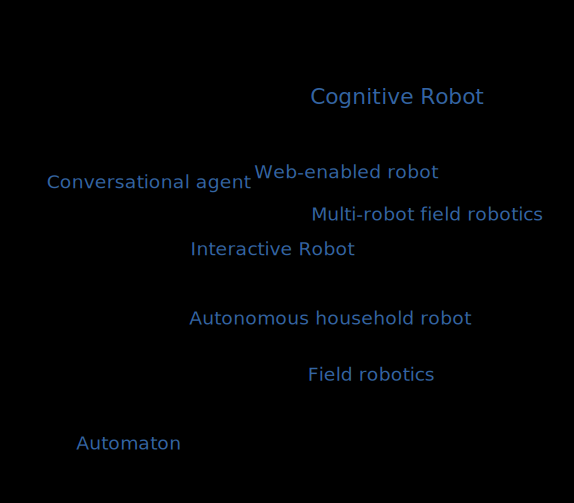
\includegraphics[width=0.7\columnwidth]{intro/social_skills.pdf}
    \caption{Towards the cognitive robot}
    \label{fig|cognitive-robots}
\end{figure}



\begin{itemize}
    \item to loosen the constraints on symbolic modeling of the robot
    environment by providing more expressive representation system than
    classical databases or fact repositories,

    \item to improve human-robot interaction by explicitly providing to the
    machine an interpretation frame, at least partially shared with the human.

\end{itemize}


%%%%%%%%%%%%%%%%%%%%%%%%%%%%%%%%%%%%%%%%%%%%%%%%%%%%%%%%%%%%%%%%%%%%%%%%%%%%%%%
%%%%%%%%%%%%%%%%%%%%%%%%%%%%%%%%%%%%%%%%%%%%%%%%%%%%%%%%%%%%%%%%%%%%%%%%%%%%%%%
%%%%%%%%%%%%%%%%%%%%%%%%%%%%%%%%%%%%%%%%%%%%%%%%%%%%%%%%%%%%%%%%%%%%%%%%%%%%%%%

\section{A prototypical scenario}
\label{sect|scenario}

\begin{figure*}
	\centering
	\includegraphics[width=0.9\textwidth]{intro/brownie_scenario.jpg}
	\caption{An illustration of the scenario}
	\label{fig|scenario}
\end{figure*}

The aim of this imaginary scenario (that has not been implemented, neither in
simulation nor on a robot) is to materialise early in this thesis the context
and challenges of knowledge representation and manipulation for service, social
and interactive robotics. It underlines the place, the role and the need of
knowledge in a near-future, everyday situation where several robots and humans
co-exist and cooperate. This scenario will also be a source of support examples
for later sections of the thesis.

We entitle our scenario ``the Brownie scenario'' (Figure~\ref{fig|scenario}):
Robi and Roba are two service robots, that can freely
move and pick objects around (with possibly different hardware and softwares
architectures, including different knowledge representation systems). They
cooperate with a human in a kitchen environment.

The main task of the scenario is the joint realization of a brownie, initiated
by Tom, the human: ``Let's make a brownie for tonight!''.

The scenario is successful if the task is achieved (the brownie is baked) in a
reasonable time (typically shorter than what it would have been required by the
human alone).

We voluntarily do not detail the subtasks of the scenario, neither we define
how they are shared amongst agents: our focus is on knowledge needs and flows.

A ``first-order'' analysis of this task leads to a rough partition of the
required \emph{representation} abilities:

\begin{enumerate}

	\item Representation abilities related to the execution of a complex
	spatio-temporal task,

	\item Representation abilities related to cooperation with other agents.

\end{enumerate}

% Representation of a complex task
We can further refine these categories: to prepare and bake a brownie, the
robot first needs to make sense of the term \emph{brownie} itself: what is it?
what is it used for? what is it made of? etc. We call this knowledge
\emph{common-sense knowledge} and the robot must be able not only to represent
it, but also to have access to an initial source (for instance through a
initial set of facts that are made available at startup, or via access to a
Web-based knowledge base like Wikipedia, etc.)

Once bound to the action \emph{make}, this should lead the robot to build and
represent a \emph{context}: we are in a scenario involving cooking. The context
enables the robot to retrieve more common-sense knowledge, like that actions
related to cooking often take place in the kitchen, cooking requires
ingredients, utensils and a procedure that may be provided by a recipe.

These last assertions imply several other capabilities: ``cooking often takes
place in the kitchen'' implies that representation of both uncertainty and
likelihood is desirable. The fact that cooking is associated to a place further
implies that the system models locations and is able to attach \emph{thematic
relations} to concepts (here, the likely location of the cooking action).

``cooking requires ingredients'' hints about another important feature closely
tied on knowledge manipulation: \emph{reasoning}. The robot can \emph{infers}
that cooking may require a recipe since a list of ingredients is a
pre-requisite of the cooking action, and a recipe may provide such a list.  If
we omit the ``may'', this is a typical example of first-order logic reasoning.
Many other reasoning techniques exist (including probabilistic ones -- ones
able to deal with the ``may''), we shall illustrate some of them later in this
scenario.

We mentioned that a recipe often provides a procedure (or a \emph{plan}). The
robot should be able to store this plan in a way that allow later execution.
The plan is likely to contain \emph{spatio-temporal constraints} (like ``put
the brownie in the oven for 20 min'' or ``let's cook \emph{for tonight}'') that
must be as well appropriately handled.

To make decision, a robot may also want to \emph{predict} the state of the
world after some action (``if I leave the cake 2h in the oven, it will burn'').
Such ability to project itself in future or, generally speaking, in other
possible state of the world is related to several cognitive ability and
reasoning techniques: \emph{planning}, \emph{projection}, \emph{representation
of possible worlds} and \emph{non-monotonic reasoning}, in addition to
common-sense knowledge and \emph{physics-based} reasoning (that allows for
instance to predict that an egg is likely to break if dropped).

Procedures are in addition often \emph{underspecified}: we can expect the
recipe to provide a cooking duration, but we usually do not expect the recipe
to tell us to first open the oven door, and then put the cake into it, since it
is self-evident that the door must first be opened to put the cake in the oven.
Our cognitive robot should ideally be able to detect and possibly complete such
underspecification.

% Representation feature that enable cooperation
Then, we want our three agents to cooperate. This, in turn, leads to another
set of cognitive abilities.

Cooperation in our scenario can intervene at many places. For instance, an
agent may want to inform another one about the number of eggs that are
necessary for the brownie. This \emph{helping} behaviour makes sense only if
the first agent knows that the recipient agent both needs the information but
does not know it. This in turn requires the robot to be able to model the
knowledge of the other agents: to think \emph{from the perspective} of another
agent (an idea that is related to the availability of a theory of mind, we will
come back to it later on).

Ability to communicate is one important pre-requisite to collaboration.
Communication in general requires the addresser and the addressee to share a
common interpretative framework (a shared common-sense knowledge -- or cultural
background -- and a shared context). In our scenario, the agents are working in
a kitchen. This element of context does not however suffice if, for example, an
agent asks another agent to ``give {[him]} the bowl''. Behind the symbol
``bowl'', which physical entity are we actually talking about? If we want to
talk and act on the world, this so-called \emph{grounding} operation is
essential. It is a bidirectional process: in covers the {\it top-down}
operation (from the symbol to the percept) and the {\it bottom-up} converse
(retrieval or creation of symbols from perception).

A related ability is called \emph{pre-supposition accommodation}: if one of the
agent moves behind another one, with the brownie dough in its arm, and says
``be careful, I'm behind you!'', we want the first agent to be able to
represent both symbolically and geometrically (because, for instance, if the
agent want to move, it must take into account the new obstacle) something that
is not directly perceived.

Also central to cooperation are the notions of \emph{joint intentions} and
\emph{joint goals}: to help the human during the cooking session, the robots
need to track how far they are into the recipe, what is the next step the human
is likely to go for, how task are currently split between agents, what action
is currently blocking the procedure, etc. This knowledge should let the robot
identify the intentions of other agents and create accordingly joint goals.
Hence, a knowledge representation system aiming at dealing with cooperative
behaviours is likely to have goal management structures taking explicitly into
account other agents' actions and goals.

In order to effectively share tasks, the robot must also know what it is
capable of: \emph{capability introspection} (both in term of general capability
and of immediate ability) is thus often desirable. It can be extended to
general introspection (like the ability to tell ``who I am'' or ``what do I
think of'') that may be required for the interaction.

Last but not least, our scenario assumes implicitly \emph{natural interaction}
between humans and robots (as showed by the casual style of the order ``Let's
make a brownie!''), and we want to ensure that the
knowledge available to the robot provides efficient support to the natural
language understanding (for instance by adopting models and vocabulary that are
both well suited for machine processing and remain as close as possible to the
humans own structures and vocabulary), and also to \emph{non-verbal forms of
communication}, like gestures.


We have emphasised several keywords in this scenario: we will come back to them
in chapter~\ref{chapt|krs} to explain them formally, and relate them to each
other. Before that, we would like to briefly focus on the challenges
specifically related to the human-robot interactions. Not only in term of
knowledge representation, but more broadly in term of specific cognitive
capabilities.

%%%%%%%%%%%%%%%%%%%%%%%%%%%%%%%%%%%%%%%%%%%%%%%%%%%%%%%%%%%%%%%%%%%%%%%%%%%%%%%
%%%%%%%%%%%%%%%%%%%%%%%%%%%%%%%%%%%%%%%%%%%%%%%%%%%%%%%%%%%%%%%%%%%%%%%%%%%%%%%
%%%%%%%%%%%%%%%%%%%%%%%%%%%%%%%%%%%%%%%%%%%%%%%%%%%%%%%%%%%%%%%%%%%%%%%%%%%%%%%

\section{Robots for interaction}
\label{sect|hri-context}

This work comes indeed from researches in the specific context of the
human-robot interaction, or, to put it another way, in the context of
interaction for \emph{joint action} with human,  in a \emph{situated}
environment (figure~\ref{fig|aperitif}).

\begin{figure}%[!ht] 
    \centering
    \includegraphics[width=0.8\columnwidth]{intro/aperitif_time.jpg} 

    \caption{Interacting with the robot in an everyday situation: the human
    asks for help in vague terms, the robot takes into account the human's {\it
    a priori} knowledge and spatial perspective to refine its understanding of
    the question.} 

    \label{fig|aperitif} 
\end{figure}

{\em \emph{Let's bake a brownie for tonight!}, proposes Tom. The robots
smoothly prepare all the ingredients, and they start to cook together a
delicious cake...}

Natural interaction and cooperation are actually the current (dare we say,
\emph{short-term}) targets for the human-robot interaction community.  The
``Brownie scenario'' we presented above belongs to the broad class of
\emph{interactive manipulation problems}: several agents agree on a (more or
less implicit) joint goal that requires some sort of cooperation to be
successfully achieved. This class of problems involves both dialogue and
manipulation and is often not completely defined at start-up: it requires
iterative, interactive resolution (step-by-step process,
questions-answers,...).

What are the cognitive prerequisites for such a sentence --``Let's make a
brownie for tonight''-- to be understood by the robot, correctly interpreted in
the spatial and temporal context of the interaction, and eventually transformed
into a set of actions? We distinguish~\cite{Lemaignan2012} four successive
steps:

\begin{enumerate}

    \item how to build and maintain a consistent geometric model of the current
        situation, acquired through perception or deduction from previous
        perceptions,

    \item how to build an unambiguous symbolic representation of concepts
        (objects, agents, actions...) underlying the interaction, and practical
        for decision-making processes,

    \item how to establish the joint goal(s), how to build and maintain
        iteratively shared (human-robot) plans, 

    \item how to refine and execute the computed plans, and how to monitor
        those achieved by its human partner?

\end{enumerate}

This work focuses on the second point: it presents techniques, developed and
used on several real robots, for the symbolic representation of environment
models suitable for grounded situation interpretation, decision-making and
control.

The other items are of course equally important to actually perform the
interaction, and we will also present (and illustrate in experiments) how our
knowledge representation system integrates and communicates with other
processes to form a \emph{knowledge-enabled} robotic architecture.


\begin{figure}
    \centering
    \includegraphics[width=0.9\columnwidth]{intro/grounding_robot.pdf}
    \caption{A robot reasoning about human-robot interaction and anticipation
    of human activities: sources of knowledge are multi-modal dialogue and
    observation of the environment and the human activities.}
    \label{fig|hri-dec}
\end{figure}


Figure~\ref{fig|hri-dec} summarises the main aspects of the interaction.
From the robot perspective, several cognitive skills are involved: dialogue
processing through verbal and deictic modalities (what does the human say? What
attitude -- glances, postures, gestures... -- does he express?), acquisition
and maintenance of one or several models of the environment, not only from the
robot point of view, but also from the other agents' points of view,
anticipation (what are the intentions of the human? Can I predict and
anticipate his/her actions?), planning and control (how would I proceed further
towards the goal?), monitoring of the other agents' activities (do we have an
effective cooperation?) and the overall progress of the task. 

As we shall see, all these cognitive capabilities also translate into
requirements on the knowledge representation systems that we want to clarify.

\begin{figure}%[!ht]
\centering
  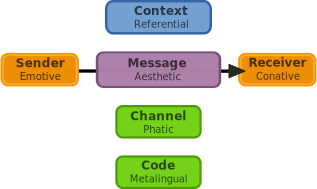
\includegraphics[width=0.6\linewidth]{communication/jakobson_communication_model.pdf}

  \caption{The \emph{Communication Model}, as proposed by
  Jakobson~\cite{Jakobson1960}. In bold characters are the \emph{communication
  dimensions}, in italics, the corresponding \emph{communication functions}.}
  
  \label{fig|jakobson_communication_model}
\end{figure}


The need of communication is probably the most salient one. The classical model
of communication proposed by Jakobson in 1960
(figure~\ref{fig|jakobson_communication_model}) exposes in a bright way the
main functions involved in a communication, be it verbal or non-verbal. While
the \emph{channel} and the \emph{code} are the technical side of the
communication, the \emph{message} in relation with the \emph{context} are
directly concerned with the question of the \emph{meaning} which itself as
tight links with the knowledge available to the agent.

The question of the communication between a robot and another agent (in a broad
way: another robot, an human, but also a remote knowledge base or the robot's
developer) underlies many of the challenges of knowledge representation: how to
represent the knowledge I want to exchange, and how to recognize, represent and
share a context that ensures both the end of the communication channel
correctly interpret the message. Or, to put it another way: how to ensure the
\emph{meaning} is correctly carried around while conducting social
interactions.

%%%%%%%%%%%%%%%%%%%%%%%%%%%%%%%%%%%%%%%%%%%%%%%%%%%%%%%%%%%%%%%%%%%%%%%%%%%%%%%

\section{The Challenges}
\label{sect|challenges}

From the set of questions raised in the previous paragraphs, we can now
articulate the challenges that are to be tackled in this field of knowledge
representation for service/companion robotics.

The first challenge is to... clarify the challenges (!) of knowledge
representation: we say ``knowledge'', we say ``reasoning'', we say
``representation'', but clear definitions are yet to be provided. Numerous
requirements on what Newell calls the \emph{knowledge level} of intelligent
agents have emerged from our \emph{Brownie} scenario, but how do they
articulate? And are they comprehensive?

To further develop what is widely known as the ``cognitive robotics'', we think
it is mandatory to lay down solid theoretical and practical foundations to the
knowledge needs of service/interactive robots. This is our first challenge.

The second challenge is more technical: how to build such a
``knowledge-enabled'' robot? Since many years, research has started to create
and study so-called cognitive architectures. Robots, as embodied and
interactive agents, raise specific issues. What are they? Which are the right
technical approaches? Can we build today such a cognitive system, and if we can
not, why that? How the abstract idea of knowledge translates into  practical,
meaningful concepts?

Our third challenge relates to the specific question of the human-robot
interaction: the robot enters the realm of a social individuality. What does
that mean? Which consequences does that have on our initial knowledge
challenge? How does it translate into practical issues, like natural language
understanding?

All the contributions (summarised in the next section) of this thesis can be
related to one of these three challenges, and hopefully contribute to the
advancement of the understanding of these questions.

%%%%%%%%%%%%%%%%%%%%%%%%%%%%%%%%%%%%%%%%%%%%%%%%%%%%%%%%%%%%%%%%%%%%%%%%%%%%%%%


\section{Contributions}
\label{sect|contributions}

We have presented our challenges: this section now summarises the main
contributions of the thesis, both from a scientific point of view and from a
technical point of view.

\subsection{Scientific contributions}
\label{sect|scientific-contributions}

The need of a better understanding of the knowledge needs of robotic
applications in human, \ie complex, dynamic, semantically-rich, environments,
is the starting point of our thesis.

Building upon an extensive review of the literature and the formulation of
several interaction scenarii (that themselves led to experiments on real
robots), we have iteratively refined the ``knowledge for interaction'' problem.
The formalization of this question is one of the main scientific outcomes of
this work: we have listed and organized into a typology a set of desirable
characteristics of knowledge representation systems for service robotics.

This typology aims at offering a comprehensive and consistent base to evaluate
existing systems and to draw new research perspectives. It also enables to
better assess the progresses of the Service Robot and Human Robot Interaction
research communities towards the long term goal of \emph{human-level artificial
intelligence} for robots, as would say McCarthy.

Another scientific contribution of this thesis is its participation to
narrow down the gap between research on embodied and disembodied artificial
agents: we have tried to bridge experiences learned from years of research on
disembodied cognitive architectures (both from the computing science and
neuropsychology communities) with the constraints from real-world systems that
weigh on robotic architectures. Notably, we have tried to identify
theoretical reference contributions from the diverse fields of cognitive
sciences that are relevant to \emph{knowledge-enabled} robotics. We have also
proposed reference implementations on robots for some of them.

At the architectural level, our work also helps to better understand the
knowledge flows in modern cognitive architectures for robots. By introducing
\emph{explicit} knowledge in our architectures, it allows the humans that
design and program robots to \emph{talk about} and question this knowledge: it
singularises and materialises concepts that were beforehand often
diffuse and ubiquitous. This leads us to define the idea and propose an
implementation of a \emph{knowledge-oriented} architecture.

This work has also several more focused scientific contributions. The
centralized semantic architecture that we propose is original. While it
exhibits shortcomings for some cognitive tasks, it also proposes novel efficient
ways to represent and manipulate knowledge simultaneously for multiple agents.
Along with the survey of current knowledge systems that we have conducted,
it effectively completes the panorama of available designs of knowledge
representation systems.

Amongst the cognitive abilities that our developments have enabled, a
particular scientific focus was led on the acquisition and modeling of
multiple, agent-dependent symbolic worlds. This opened new perspectives related
to \emph{perspective-aware} reasoning or \emph{theories of mind} for robots
that are detailed in this work.

We also have a scientific contribution on the grounding of human-robot
dialogue in natural language. We have algorithmically formalized a novel
grounding process that takes advantage of multi-modal communication (verbal,
deictic and immanent) and handles the semantics of several more complex
language features like quantification. This system also has contributions
related to the semantic validation of thematic roles and interactive
disambiguation that takes into account human attentional focus.

\subsection{Technical contributions}
\label{sect|technical-contributions}


This thesis has four major technical contributions: the software development of
\emph{ORO server} as a semantic blackboard dedicated to robotic applications,
the design of the \emph{ORO ontology} as a domain-specific common-sense
ontology tailored for service robotic needs, the pervasive integration of a new
semantic layer into several existing robot architecture, and finally, the
software development of \emph{Dialogs}, a novel module for natural language
grounding.

The main software contribution of the thesis is the development of an
open-source, versatile and light-weight knowledge base that stores in a
formal framework based on first-order logics both the robot's own beliefs and
the mental models of every other cognitive agents that the robot interacts
with. This tool, called \emph{ORO}, is implemented as a
platform/middleware-agnostic server, and exposes to the robot's modules
several advanced reasoning services (via the integration of external
reasoners). This software project is now publicly available, used by other
laboratories, and comes with extensive documentation and bindings for several
mainstream languages (C++, Python...) and middlewares (ROS, YARP).

In parallel of this development, and in collaboration with other developers,
we have also drafted (and partially implemented) a proposal for a standard API
for knowledge manipulation that supports the specific needs of robotic
applications.

Coming along with the ORO server, we introduce in this thesis the
\emph{ORO common-sense ontology} which is a proposal of an upper ontology for
service and interactive robotics. This ontology consists of about two hundred
classes, relations and rules that are relevant for the modeling of the
robot's beliefs and state, and the interactions with other agents (humans or
robots). This ontology also tries to stay closely aligned with the standard
{\sc OpenCyc} upper-ontology to guarantee interoperability with semantic
web resources and other robots.

A third technical contribution is the introduction of a new
knowledge-oriented, event driven communication model between high-level
decisional modules: by introducing the concept of \emph{semantic events}, the ORO
server enables the development of new executive layers that combine reactive
behaviour with high-level abstractions: for instance, triggering a behaviour
when a human looks at the robot while sit, can be expressed in our architecture
as a single proposition: {\tt subscribe([* type Human, * looksAt myself, *
isSitting true], behaviour\_callback())}. This highly expressive event model
opens new ranges of development opportunities for decisional modules.

During the preparation of the thesis, we have also developed a new stand-alone
natural language processor for English language. It takes advantage of the
different symbolic models exposed by the ORO server to analyse, resolve the
semantics and ground dialogues. It can process orders, questions and positive
assertions and translates them into new symbolic facts. It includes a custom
grammatical parser, a re-verbalization module, several discrimination
strategies, including interactive ones. The application is developed in Python
(about 15K lines of code), can be used in real-time on the robot, and is
accompanied by a speech recognition interface developed as an Android
application.

A last notable software contribution is our involvement in the MORSE simulator
for academic robotics. We have played a central role in the original design and
development of the core functionalities of this open-source simulator which is
now used by over twenty laboratories world-wide. While this project as a whole
is not directly related to the thesis main domain, we have led the effort towards
effective simulation of human-robot interaction in MORSE, which is now the
current state-of-the-art in this domain. It is briefly presented at
section~\ref{sect|simulation}.


%%%%%%%%%%%%%%%%%%%%%%%%%%%%%%%%%%%%%%%%%%%%%%%%%%%%%%%%%%%%%%%%%%%%%%%%%%%%%%%
%%%%%%%%%%%%%%%%%%%%%%%%%%%%%%%%%%%%%%%%%%%%%%%%%%%%%%%%%%%%%%%%%%%%%%%%%%%%%%%
%%%%%%%%%%%%%%%%%%%%%%%%%%%%%%%%%%%%%%%%%%%%%%%%%%%%%%%%%%%%%%%%%%%%%%%%%%%%%%%


\section{A reader's guide}

\subsection*{The thesis in 15min}

Because of the contingencies of this world, we acknowledge that the complete
reading of this thesis may not fit in one's tight schedule.

If you have only about 15 minutes to dedicate to this work, we suggest to read
the following sections in that order:

\begin{itemize} \item What are the challenges? (section~\ref{sect|challenges},
            page~\pageref{sect|challenges}),

    \item Contributions (section~\ref{sect|contributions},
        page~\pageref{sect|contributions}),

    \item The ORO functional overview (section~\ref{sect|functional-overview},
        page~\pageref{sect|functional-overview}),

    \item The first interaction experiment (section~\ref{sect|expe1},
        page~\pageref{sect|expe1}),

    \item The evaluation of ORO and other knowledge representation systems
        (section~\ref{sect|evaluation-oroserver},
        page~\pageref{sect|evaluation-oroserver}),

    \item And finally, the discussion on perspectives
        (section~\ref{sect|perspectives}, page~\pageref{sect|perspectives}),

\end{itemize}

Hopefully, this quick overview of this work can help you to go in depth into
the sections relevant to your concerns.

\fxfatal{Re-read these sections to make sure it makes sense}

\subsection*{For the patient reader}

Roughly speaking, the thesis is organized in three parts: an analysis of
knowledge representation systems for service and personal robotic, the
presentation of ORO, our own implementation of such a knowledge representation
system, and finally we report on practical uses of explicit knowledge
manipulation on robots, first for natural language processing, then through
several experiments.

The first part is covered in the chapter~\ref{chapt|krs}: after a discussion on
what we call ``knowledge'' in our context, we explore its importance by
listing, in a typology of characteristics, the requirements of our robots
related to knowledge management. This first chapter is completed by a survey of
eight systems for knowledge management that have been already deployed on real
robots.

At the end of the thesis, we give a second look at these systems to try to
draw a picture of the overall landscape of knowledge representation approaches
in the robotic reseach community, to identify new possible research directions.

The second part is covered by chapters~\ref{chapt|oroserver} and
\ref{chapt|implementation-integration}. Chapter~\ref{chapt|oroserver} presents
the functional side of ORO server, some of the algorithms that are
implemented, and discusses its knowledge model (the ORO \emph{common-sense
ontology}). The technical side is presented in
chapter~\ref{chapt|implementation-integration} where we emphasise the
integration of ORO within a larger robotic architecture. The articulations with
perceptions, planning and control are presented.

Chapters~\ref{chapt|dialogs} and \ref{chapt|evaluation} form the third and last
part of the thesis. Chapter~\ref{chapt|dialogs} details \emph{Dialogs}, a
module for situated dialogue grounding that takes advantage of the symbolic
knowledge exposed by ORO, and chapter~\ref{chapt|evaluation} presents
several evaluations of our work through various experiments conducted during
the four years of the thesis preparation.

We conclude the thesis with a discussion of several issues related to knowledge
management in service robots (importance of embodiement, relationships between
the symbolic and continuous realms, etc.) and some remarks that could further
improve knowledge representation and management in future robotic
architectures.


\chapter{Symbolic knowledge representation}

\section{Which end for knowledge representation?}
\label{sect|krs-purpose}

\subsection{Limits of traditional representation systems for robotics}
\label{subssect|limits}

\subsection{Specific requirements of robotics}
\label{subssect|robotics-specifics}

\subsection{Benefits of a symbolic knowledge representation system}
\label{subssect|krs-benefits}

\section{Formalisms for symbolic representation}
\label{sect|formalisms}

\section{Designing the \textsc{OpenRobots} common-sense ontology}
\label{sect|commonsense-design}

\section{Evaluation of a symbolic representation }
\label{sect|krs-evaluation}


\chapter{oro-server, a symbolic knowledge representation system for robotics}
\label{chapter|oroserver}

This chapter introduces the \emph{OpenRobots Ontology} server and its
common-sense knowledge base.

We present a \textbf{functional description} of oro-server, and detail at
lenght its knowledge model. Its actual implementation is discussed in the next
chapter.

We also present in depth the \emph{OpenRobots Common-Sense Ontology} that
contains most of the knowledge at hand when the robot starts.

\section{Functional overview}
\label{sect|functional-overview}


We have adopted a centralized approach for knowledge management called
ORO~\cite{Lemaignan2010}. The platform is designed as a central
knowledge storage service implemented as a server where the robot
components can add or query statements at run-time. Figure~\ref{fig|oro-overview}
illustrates the main functional components of ORO.

\begin{figure}
\centering
  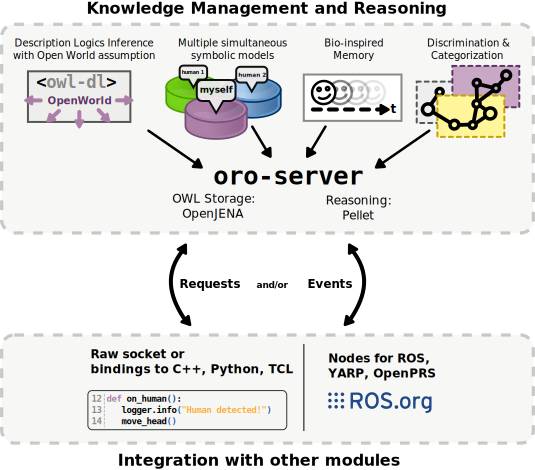
\includegraphics[width=0.8\linewidth]{oroserver/oro_architecture_functional.pdf}
  \caption{Overview of the ORO architecture.}
  \label{fig|oro-overview}
\end{figure}

At the core, ORO is build around the
OpenJena\footnote{\url{http://www.openjena.org}} ontology management library,
connected to the Pellet\footnote{\url{http://clarkparsia.com/pellet}}
reasoner.

A front-end accepts and manages connections to clients. The clients' requests
are processed by a set of internal modules: basic operations on statements,
but also higher cognitive and human-robot interaction related functionalities
are available. External plugins can also be easily added.

Besides acting as a facts database, the ORO platform exposes several
functions: operations on knowledge statements relying on inference (through a
continuous first-order logic classification process), management of
\emph{per-agent} symbolic models, and also higher cognitive and human-robot
interaction related functionalities like categorization of sets of concepts
or profiles of memory (that enable the robot to ``forget'' about some facts).

ORO also provides an event mechanism that allows components to be triggered
when specific events occur. A component can for instance subscribe to events
of kind \setstmt{?agent isVisible true, ?agent type Human}. As soon as the
perception layer detects a human in the robot's field of view and accordingly
updates the knowledge base, the executive layer is triggered. The event
framework also takes advantage of the inference capabilities of ORO. Thus an
event can be indirectly triggered if its triggering conditions can be
inferred to be true.


%%%%%%%%%%%%%%%%%%%%%%%%%%%%%%%%%%%%%%%%%%%%%%%%%%%%%%%%%%%%%%%%%%%%%%%%%%%%%%%
%%%%%%%%%%%%%%%%%%%%%%%%%%%%%%%%%%%%%%%%%%%%%%%%%%%%%%%%%%%%%%%%%%%%%%%%%%%%%%%
%%%%%%%%%%%%%%%%%%%%%%%%%%%%%%%%%%%%%%%%%%%%%%%%%%%%%%%%%%%%%%%%%%%%%%%%%%%%%%%

\section{The ORO Knowledge model}
\label{sect|knowledge-model}

\subsection{Expressiveness: What Can be Represented?}
\subsubsection{Open World and Close World Assumptions}
\subsubsection{Meta-cognition: knowledge on the knowledge}
Narrower, more technical dimension of the introspection.

%%%%%%%%%%
\subsection{How things are represented?}
\subsubsection{Role Representations}
Spatio-Temporal Representations:

\paragraph{Representation of time}
\paragraph{Representation of space}
\paragraph{Representation of events and actions}

\subsubsection{Context modeling}
\subsubsection{Possible-Worlds and representing what others know}

\paragraph{Multi-model representation for Persepective-taking}
\label{sect|alterite}

...

We present at section~\ref{sect|perspectivetaking}, page~\pageref{sect|perspectivetaking} an 3D real-time environment, SPARK, that allows to compute on-line several perspective aware symbolic properties.

\subsection{False beliefs and Theory Of Mind}
\label{sect|theory-of-mind}



\subsubsection{Introspection: Who am I? What can I do?}

%%%%%%%%%%
\subsection{Reasoning Techniques}

\subsubsection{Standard reasoning techniques}


Knowledge is stored as OWL/RDF ontologies in ORO. We use the Pellet reasoner to
classify them. This enables several type of reasoning:

\begin{itemize}
	\item reasoning on inheritance relations (\eg \emph{all bottles are containers}),
	\item property axioms
		\begin{itemize}
		\item entailments based on predicates' domain and range,
		\item cardinality constraints (including \concept{allValue}, 
		\concept{someValue}, \concept{hasValue}),
		\item property characteristics (symmetry, transitivity)
		\end{itemize}
	\item class restrictions like: \par \footnotesize \concept{Bottle} $\equiv$
		\concept{Artifact} {\bf that} (\concept{hasShape} {\bf value}
		\concept{cylinderShape})\footnote{This example uses the \emph{Manchester
		syntax}, \url{http://www.w3.org/TR/owl2-manchester-syntax/}} \normalsize
	\item set operations like: \par \footnotesize \concept{Color} $\equiv$ {\bf unionOf}(\concept{blue},
		\concept{green}, \concept{orange}, \concept{black}...) \normalsize
	\item generic SWRL ({\em Semantic Web Rule Language}) rules like: \par
		\footnotesize \concept{looksAt(?agt, ?obj)} $\land$
		\concept{pointsAt(?agt,?obj)} \par $\Rightarrow$ \concept{focusesOn(?agt, ?obj)}
		\normalsize 
	\end{itemize}

We provide in ORO accessors to query, add or remove all these properties and
restrictions (except the SWRL rules) at run-time. This allows knowledge
introspection and enables the robot to alter its own knowledge structures (the
so-called \emph{T-Box} model) during its life-time by adding new constraints
and properties to classes and predicates (we can for instance teach the robot
\emph{at runtime} that cats are animals, \ie \stmt{Cat rdfs:subClassOf
Animal}).


\paragraph{Decidability}

...


\subsubsection{Reasoning with uncertainty}
\subsubsection{(Non) Monotonic Reasoning}


\subsubsection{Memory}
\label{subssect|memory}


\subsubsection{Learning by modifying the knowledge structure}

%%%%%%%%%%%%%%%%%
\subsection{The left-overs: What ORO does not provide?}

\subsubsection{Representation of uncertainty and likelihood}

\subsubsection{Presupposition accommodation}
\subsubsection{Prediction, projection and diagnosis tasks}
\paragraph{Projection task}: determining whether or not some condition while
hold after a sequence of actions.

\paragraph{Legality task}: determining whether a sequence of action can be
performed starting in some initial state.

\paragraph{Diagnosis}: this corresponds to the ability to rewind on past events
in case of failure to provide possible explanation. This can be seen as the
temporal reverse of the projection task.


\subsubsection{Physics-based reasoning}
\subsubsection{Planning}
Making decision based on prediction




%%%%%%%%%%%%%%%%%%%%%%%%%%%%%%%%%%%%%%%%%%%%%%%%%%%%%%%%%%%%%%%%%%%%%%%%%%%%%%
%%%%%%%%%%%%%%%%%%%%%%%%%%%%%%%%%%%%%%%%%%%%%%%%%%%%%%%%%%%%%%%%%%%%%%%%%%%%%%
%%%%%%%%%%%%%%%%%%%%%%%%%%%%%%%%%%%%%%%%%%%%%%%%%%%%%%%%%%%%%%%%%%%%%%%%%%%%%%

\section{Knowledge instanciation: the OpenRobots Common-Sense Ontology}

How much knowledge is available? Which content? How big is the knowledge base?

\subsection{Designing the \textsc{OpenRobots} common-sense ontology}
\label{sect|commonsense-design}



\chapter{Implementation and Integration in Robots}
\label{chapter|implementation_integration}

\section{Some implementation notes}

This section presents some of the main technological choices that have
been made to implement the knowledge base.

Some of the main algorithms are presented here as well (like the algorithms for clasification and discrimination,~\ref{sect|discrinimation}).

\subsection{A centralized server-based implementation}
\label{sect|oro-serverbased}


\subsection{OWL-DL ontologies and Jena}
\label{sect|jena}

\subsection{Reasoning: the Pellet reasoner}
\label{sect|pellet}

\subsection{Classification and discrimination algorithms}
\label{sect|discrimination}

%%%%%%%%%%%%%%%%%
\section{Bindings to other components/languages}
\label{sect|interfacing}

%%%%%%%%%%%%%%%%%
\section{Monitoring and debugging}
\label{sect|monitoring}

\subsection{Logging}

\subsection{Vizualisation}

oro-view, DOT export...

%%%%%%%%%%%%%%%%%
\section{Integration in the robot architecture}

\subsection{RPC and events-oriented interactions}

\subsection{Acquiring and Anchoring Knowledge in the physical world: the SPARK module}

\subsubsection{Building an Agent-Aware Symbolic Model of the Environment}
\label{sect|situ}

Anchoring perceptions in a symbolic model requires perception abilities and
their symbolic interpretation. In this section we present SPARK (\emph{SPAtial
Reasoning \& Knowledge}~\cite{Sisbot2011}), a situation assessment reasoner
that generates relevant symbolic information from the geometry of the
environment with respect to relations between objects, robots and humans.

\begin{figure}[ht!]
   \begin{center}
%
       \subfigure{
           \includegraphics[width=0.5\textwidth]{spark/etat.jpg}
       }%
       \subfigure{%
          \includegraphics[width=0.43\textwidth]{spark/etat_spark.png}
       }\\ %  ------- End of the first row ----------------------%
%
   \end{center}

   \caption{The robot represents at runtime its environment in a 3D model
   resulting of the sensors' inputs fusion (Kinect, motion capture, 2D barcodes
   tracking).}

   \label{fig|spark}

\end{figure}

Figure~\ref{fig|spark} shows a screenshot of the SPARK environment side-by-side
with the real environment: as mentioned in the introduction, objects are
identified and localized through 2D barcodes. The human pose is tracked with
a Microsoft Kinect device (assisted by motion capture to accurately track the
head motion, which is required to compute what the human is looking at).

This geometric model is continuously updated at runtime by the robot.

\paragraph{Symbolic locations}

Human commonly refer to the positions of objects with symbolic descriptors
(like \emph{on}, \emph{next to}...) instead of precise, numeric position. These
type of descriptors have been studied in the context of language grounding
(\cite{O'Keefe1999,Matuszek2010,Regier2001,Kelleher2006,Blisard2005}). In this
work we focus agent-independent symbolic locations and agent-dependent,
relative locations.

\paragraph{Agent-independent locations}

We can refer to object locations with respect to other objects in the
environment, such as \emph{above, next to, in}, etc. In this work we compute
three main relations based on the bounding box and center of mass of the
objects (fig.~\ref{fig|sprelations}): 

\begin{itemize}
	\item \concept{isOn}: computes if an object $O_1$ is on another object $O_2$ by
	evaluating the center of mass of $O_1$ according to the bounding box of $O_2$.

	\item \concept{isIn}: evaluates if an object $O_1$ is inside another object
	$O_2$ based on their bounding boxes $BB_{O_1}$ and $BB_{O_2}$.

	\item \concept{isNextTo}: indicates whether an object $O_1$ is next to another
	object $O_2$. We cannot use a simple distance threshold to determine if two
	objects are next to each other since the relation is highly dependent on the
	dimensions of the objects. For instance, the maximum distance between large
	objects (\eg two houses) to consider them as being next to each other is much
	larger than the maximum distance we would consider for two small objects (\eg
	two bottles). Thus, the relation between the dimensions and the distances of
	the objects are taken into account.  

\begin{figure} 
	\centering
	\includegraphics[width=0.95\columnwidth]{spark/spatial_relation.pdf}
	\caption{Spatial relations between two objects: (a) \concept{isOn} relation, 
	(b) \concept{isIn} relation, and (c) \concept{isNextTo} relation.} 
	\label{fig|sprelations} 
\end{figure}

\end{itemize} 

To ensure the different agent models are up-to-date, all these properties are
always computed on-line, each time the current state of the world changes.

Table~\ref{facts|sprelations} lists all the symbolic relationships that are
currently computed by the system.

\begin{table}[h]
    \centering
    \begin{tabular}{p{1.5cm}p{5cm}p{2cm}p{2.7cm}}
	\rowcolor{white}
    \textbf{Subject} & \textbf{Predicate} & \textbf{Object} & \emph{Notes} \\ 
    \hline
	 \concept{Location} & \concept{isAt} $\equiv$ \concept{cyc:objectFoundInLocation}  &  \concept{Location} & \\ 
	 &  $\rightarrow$ \concept{isOn} $\equiv$ \concept{cyc:above\_Touching}  &  & \\ 
	 &  $\rightarrow$ \concept{isIn}  &  & \\ 
	 &  $\rightarrow$ \concept{isNextTo}  & &  \\ 
	 \concept{Location}  & \concept{isAbove} $\equiv$ \concept{cyc:above-Generally}  &  \concept{Location}  &  inverse of \concept{isBelow} \par \concept{isOn} $\Rightarrow$ \concept{isAbove}\\ 
	 \concept{Location}  & \concept{isBelow}  & \concept{Location}  &  inverse of \concept{isAbove}
	\end{tabular}

	\caption{List of statements describing spatial relationships between
	objects. ``$\rightarrow$'' indicates sub-properties. When existing, the
	equivalent predicate in the {\sc OpenCyc} standard (prefix \concept{cyc:})
	has been added.}

\label{facts|sprelations}
\end{table}

SPARK also compute symbolic facts related to agent independent world dynamics.
The predicate \concept{isMoving} states, for each tracked entity, whether it is
currently moving or not.


\paragraph{Agent-dependent placements}

While in previous section we listed several \emph{absolute} location predicate,
many topological relations are directly dependent from the observation point.

The predicate \concept{hasRelativePosition} represents spatial locations
between agents and objects that are agent dependent.  For example we say ``it
is on my right, on your left, ...'' We compute these spatial locations by
dividing the space around the referent (an agent) into $n$ regions based on
arbitrary angle values relative to the referent orientation.  For example, for
$n = 4$ we would have the space divided into \emph{front, left, right} and
\emph{back}. Additionally, two proximity values, \emph{near} and \emph{far},
may also be considered. The number of regions and proximity values can be
chosen depending on the context where the interaction takes place.


To build an agent-dependent model of the world, \emph{Perspective
Taking}~\cite{Flavell1992,Tversky1999} is employed by the reasoner to provide
the robot with the ability to put itself at the human's place (by moving a
camera in the geometric model) and to reason about the world from different
perspectives.


Through perspective taking, SPARK computes for each agent a symbolic
description of the relative positioning of objects in the environment (table
\ref{facts|relative}).

\begin{table}[h]
	\centering
	    \begin{tabular}{p{1.5cm}p{6cm}p{1.5cm}l}
		\rowcolor{white}
		\textbf{Subject} & \textbf{Predicate} & \textbf{Object} & \emph{Notes} \\
		\hline
	 \concept{Location}  & \concept{hasRelativePosition}  & \concept{Location} & \\ 
	 & 	$\rightarrow$ \concept{behind} $\equiv$ \concept{cyc:behind-Generally}  &  & inverse of \concept{inFrontOf}  \\ 
	 &  $\rightarrow$ \concept{inFrontOf} $\equiv$ \concept{cyc:inFrontOf-Generally}  & 	 & 	 inverse of \concept{behind}  \\ 
	 &  $\rightarrow$ \concept{leftOf}  &  &  inverse of \concept{rightOf} \\ 
	 &  $\rightarrow$ \concept{rightOf}  & 	 & 	 inverse of \concept{leftOf}  \\ 
	 \concept{Object}  & \concept{cyc:farFrom}  &  \concept{Agent} & \\ 
	 \concept{Object}  & \concept{cyc:near}  &  \concept{Agent} & 
	\end{tabular}
	\caption{List of statements describing relative spatial relationships between objects and agents.}
	\label{facts|relative}
\end{table}


\subsubsection{Building a Model of Agents}
\label{sect|grounding_agents}

Building a grounded symbolic model of the physical environment does not suffice
in general to fully ground the human-robot interaction.

We divide the process of building models for agents into two categories:
operations related to the assessment of the current situation (for instance,
\emph{What does the human do? What does he see?}), and operations related to
the estimation of potential actions (for instance, \emph{Which regions could
the human reach if I want to hand over an object?}). We call these
potentialities of action \emph{Mightabilities}.

\paragraph{Agent Capabilities}

There are a number of common properties for a robot and a human related to
their capabilities in a given situation: they can both reach, grasp, look at,
point at, etc.: we group them in the \emph{Agent} category, defined as entities
that can act in the environment and manipulate it.

In this work we focus on the following capabilities from each agent's
perspective:

\begin{itemize}

\item \emph{Sees}: An important ability to know about an agent is to predict
\emph{What can it see?}, \ie what is within its field of view (FOV). A robot being
able to compute this information can then act accordingly. An example would be
a clarification scenario where the human is searching for an object and the
robot is able to infer that he/she is looking for the one that is not visible
(otherwise the user would not be searching for it).  In
Figure~\ref{fig::sparkRepresentations}\emph{a} the field of view of a person is
illustrated with a grey cone (broader one). While he is able to see the two
small boxes on the table in front of him, the big box on his right is out of
his FOV, and therefore, he is not able to see it. 

\item \emph{Looks At}: this relation corresponds to what the agent is focused
on, \ie where its focus of attention is directed. This model is based on a
narrower field of view, the field of attention (FOA). 
Figure~\ref{fig::sparkRepresentations}\emph{a}
shows the field of attention of a person with a green cone (narrower one). In
this example only the grey box satisfies the \concept{looksAt} relation.

\item \emph{Points At}: verifies whether an object is pointed at by an agent.
This relation is particularly useful during interaction when one of the agents
is referring to an object saying ``this" or ``that" while pointing at it.
 
If a larger object occludes a smaller one while an agent is pointing at them, the
outcome of the evaluation will result only in one relation, \ie \stmt{agent\_01
pointsAt object\_01} since the small one is not visible to the agent.  On the
contrary, if the small object is in front of the big one, then both objects
will satisfy the relation, which may generate an ambiguity (which object the
agent refers to?) that should be solved through higher level reasoning (\eg
context analysis or clarification through verbal interaction).

\item \emph{Reachable}: it allows the robot to estimate the agent's capability
to reach an object, which is fundamental for task planning. For example, if the
user asks the robot to give him/her an object, the robot must compute a transfer
point where the user is able to get the object afterward. 
Figure~\ref{fig::sparkRepresentations}\emph{b} shows different reachability postures for each object
on the table. In the example, the bottle and the box are both reachable for the
human, but the teddy bear is too far. Instead, from the robot's perspective,
the teddy bear is reachable, while the bottle is not.

\end{itemize}

\begin{figure*}[!t]
	\begin{center}
	\subfigure[]{
		\includegraphics[width=0.4\linewidth]{spark/looks.jpg} 
	}
	\subfigure[]{
		\includegraphics[width=0.35\linewidth]{spark/reach.jpg}
	} 
	\caption{(a) Field of view (FOV) and the field of attention (FOA) of the human. (b) Different reaching postures for the human.}
	\label{fig::sparkRepresentations}
	\end{center}
\end{figure*} 


While the first three relations (\concept{sees}, \concept{looksAt} and
\concept{pointsAt}) are computed through a model based approach, the latter one
is based on the Generalized Inverse Kinematics with pseudo inverse
method~\cite{Nakamura90,Baerlocher04} to find a posture for the
agent where its end-effector is at the center of the object within a given
tolerance.

Tables~\ref{facts|capabilites} summarizes the predicates produced by SPARK
during the agent capabilities analysis phase.

\begin{table}[h]
	\centering
		\begin{tabular}{p{2cm}p{4.5cm}p{2cm}p{3.5cm}}
		\rowcolor{white}
		\textbf{Subject} & \textbf{Predicate} & \textbf{Object} & \emph{Notes} \\
		\hline
		 \concept{Agent}  & \concept{looksAt}  & \concept{SpatialThing} \\
		 \concept{Agent}  & \concept{sees}  &  \concept{SpatialThing}  &    \\ 
		 \concept{SpatialThing}  & \concept{isInFieldOfView}  &  \concept{xsd:boolean}  & via inference: \par \stmt{myself sees *} $\Leftrightarrow$ \stmt{* isInFieldOfView true} \\ 
		 \concept{Agent}  & \concept{pointsAt} $\equiv$ \concept{cyc:pointingToward}  & \concept{SpatialThing} \\ 
		 \concept{Agent}  & \concept{focusesOn}  &  \concept{SpatialThing}  &  via inference: \par \concept{looksAt} $\wedge$ \concept{pointsAt} $\Rightarrow$ \concept{focusesOn} \\
		\concept{Agent} & \concept{seesWithHeadMovement} &  \concept{SpatialThing} \\
		\concept{Agent} & \concept{reaches} &  \concept{Object} \\ 

	\end{tabular}

	\caption{List of facts describing the attentional state and the abilities
	of an agent. \concept{looksAt} is interpreted as an object \emph{being in
	the field of attention} of an agent. An object is \concept{see}n if it is
	visible for the agent without moving the head (\ie, in \emph{field of
	view}).}

	\label{facts|capabilites}
\end{table}

Table~\ref{facts|agentstate} lists the other symbolic facts that are
produced and maintained by SPARK related to the general state of the agent.

\begin{table}[h]
	\centering
	\begin{tabular}{p{2cm}p{5cm}p{2cm}}
		\textbf{Subject} & \textbf{Predicate} & \textbf{Object} \\
		\hline
		\concept{Agent} & \concept{hasIn\{Left|Right\}Hand}  &  \concept{GraspableObject} \\ 
		\concept{Agent} & \concept{hasPosture}  &  \concept{Posture} \\
		\concept{Agent} & \concept{currentlyBodilyDoes}  &  \concept{Action}
	\end{tabular}

	\caption{List of statements describing the state of an agent in general.
	\concept{Posture} can be either \concept{standing} or \concept{sitting}.
	The \concept{currentlyBodilyDoes} predicate states the current action of
	the agent, be it intentional or not.}

	\label{facts|agentstate}
\end{table}

%%%%%%%%%%%%%%%%%

\subsection{Integration with symbolic task planning and executive layers}

\subsubsection{Symbolic Task Planning}

Complex human robot interaction may necessitate a strong reasoning about the
environment and the capabilities of involved agents: How can they achieve a
specific goal? What are the required actions to achieve this goal? Which
actions can be performed by each agent? etc.

In the previous sections, we have seen how symbolic knowledge is produced and
stored from the real physical world. In this section, we present one possible
way to use these symbolic models of the environment and interacting agents to
produce a plan of actions for a complex goal.

\begin{figure}
    \centering
    \includegraphics[width=0.9\columnwidth]{integration/hatp_console.jpg}
    \caption{Screenshot of the HATP console. On the left panel, we see the
    results of the requests to ORO, on the bottom right the resulting plan.}
    \label{fig|hatp_console}
\end{figure}

In order to devise how a given goal can be accomplished, the robot has to
elaborate a plan,\ie a set of actions to be achieved by the robot and its human
partners.  This is the role of HATP \cite{Alili2008} (for Human Aware Task
Planner, figure~\ref{fig|hatp_console}).  HATP is based on a Hierarchical Task
Network (HTN) refinement, which performs an iterative task decomposition into
sub-tasks until reaching atomic actions~\cite{Nau2003}.  The planning domain
defines a set of methods describing how to decompose a task and can be seen as
the {\it how-to} knowledge of the robot.  HATP is able to produce plans for the
robot's actions as well as for the other participants (humans or robots). It
can be tuned by setting up different costs depending on the actions to apply
and by taking into account a set of constraints called social rules. This
tuning aims at adapting the robot's behavior according to the desired level of
cooperation of the robot.

\paragraph{Agents and action streams} The robot plans not only for itself but
also for the other agents. The resulting plan, called ``shared plan'' is a set
of actions that form a stream for each agent involved in the goal achievement.
Depending on the context, some ``shared plans'' contain causal relations
between the agents. For example, the second agent needs to wait for the success
of the first agent's action to be able to start its own action. When the plan
is performed, causal links induce synchronization between agents.
Figure~\ref{plan_hatp1} illustrates a plan with two streams.

\begin{figure}[htbp]
  \centering
  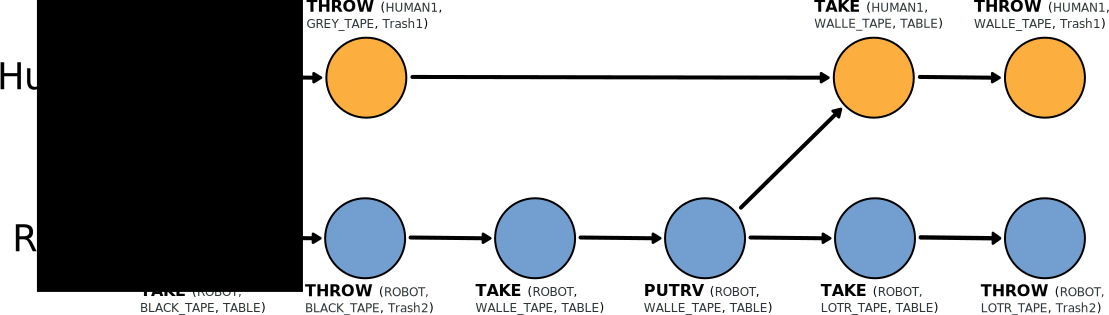
\includegraphics[width=0.8\columnwidth]{integration/hatp_plan1.pdf}
  \caption{A plan produced by HATP with 2 streams}
  \label{plan_hatp1}
\end{figure}

\paragraph{Action costs and social rules} A cost and a duration function is
associated to each action.  The duration function provides a duration interval
for the action achievement and is used, in one hand, to schedule the different
streams and, in the other hand, as an additional cost function.  In addition to
these costs, HATP also takes into account a set of social rules.  Social rules
are constraints aiming at leading the plan construction towards the best plan
according to some human preferences. The social rules we have defined so far
deal with:

\begin{itemize}

    \item undesirable state: to avoid a state in which the human could feel
    uncomfortable;

    \item undesirable sequence: to eliminate sequences of actions that can be
    misinterpreted by the human;

    \item effort balancing: to adjust the work effort of the agents;

    \item wasted time: used to avoid long delays between the actions of the
    human partner;

    \item intricate links: to limit dependencies between the actions of two or
    more agents.

\end{itemize}

\begin{figure}[htbp]
  \centering
  \includegraphics[width=0.8\columnwidth]{integration/hatp_plan2.pdf}
  \caption{A plan with the wasted time social rule}
  \label{plan_hatp2}
\end{figure}

Figure~\ref{plan_hatp2} illustrates an alternative plan to the previous one
(fig.~\ref{plan_hatp1}) if the wasted time social rule is used.  The obtained
shared plan is the best plan according to a global evaluation of these multiple
criteria.

\paragraph{Several levels of cooperation} By tuning its costs and adapting its
social rules, HATP can be used to compute various alternative plans. These
plans can be categorized into several levels of cooperation

\begin{itemize}

    \item helping the human to achieve his goal by acting for him

    \item sharing concrete resources by handing some objects

    \item collaboration of the robot and the human by coordinating their
    actions towards a human-robot joint goal.

\end{itemize}


\subsubsection{Execution Control}
\fxnote{CRAM, SHARY, pyrobots, RAD...}

\subsection{Integration with natural language processors}

%%%%%%%%%%%%%%%%%

\subsection{Towards an Event-Driven, Knowledge-Oriented Architecture}

In this section, we have presented how knowledge streams are organized between
several components: {\it(1)} {\sc ORO}, the ontology-based knowledge server
that stores and maintains classified RDF statements produced by other modules
in agent-specific models and allows information to be retrieved either through
queries or via an event system; {\it(2)} {\sc SPARK}, the grounded,
human-aware, 3D model of the environment that performs all the spatial
reasoning within this architecture, including reasoning involving motion
planing (to compute reachability of objects) and perspective taking, {\it(3)}
{\sc CRAM}, {\sc SHARY}, {\sc pyRobots}, {\sc RAD}, {\sc HATP} as different
examples of execution controllers and symbolic task planners that take
advantage of semantic abstractions provided by knowledge base and {\it(4)} {\sc
Dialogs}, a natural language processor that performs simple grammatical parsing
of English language, grounds the semantic content of the utterance (if
necessary, also interacts with the user to disambiguate), and eventually
generates a RDF representation of the sentence.

Altogether, these components compose an architecture that we call
\emph{knowledge-oriented}:

\begin{itemize} \item{Knowledge is explicitly stored in one central and
consistent repository of facts, accessible by all modules.} \item{Knowledge is
represented in a strict formalism (OWL statements) and with a clearly defined
vocabulary (stated in the {\tt commonsense.oro.owl} ontology).} \item{The first
two points enable both a loosely-coupled architecture where modules can very
easily be removed or replaced by other ones as long as they share the same
semantics (modules are defined by the knowledge they produce),} \item{and a
\emph{symbolic} reactive, event-driven approach to supervision. By managing
events at the same level as the reasoner, we take full advantage of the
inference abilities of ORO to trigger events whose \texttt{true} conditions can
be inferred.} \item{Finally, this architecture allows for the combination of
very different knowledge modalities in a single homogeneous environment,
bringing mutual benefits to components. For instance, the dialogue processing
module can perfectly run without any geometric perception, but its
disambiguation routines can transparently benefit from it when available (since
richer symbolic descriptions of objects are then available).} \end{itemize}

This architecture moves away from standard layered approaches. Interactions
between components are mostly bidirectional and, from the software components
point of view, we do not introduce layers of abstraction (we do, however, have
access to the lower level modules of the robot to execute actions, but all
cognition-related modules reside at the same level). This is especially visible
for the dialogue input processing. This component does not simply act as an
alternative perceptual input to the symbolic database, but also actively
queries previously acquired knowledge to disambiguate and validate the newly
created symbolic knowledge, as we will present in details in the following
chapter.

Regarding the anchoring question, this architecture is bidirectional. The
components we described provide a \textit{bottom-up} grounding process: SPARK
and \textsc{Dialogs} constantly build and push new symbolic contents about the
world to ORO where it becomes accessible to decisional layers. In parallel, ORO
relies on reasoning in a \textit{top-down} way to produce new facts that may
trigger in return physical behaviours. 

We believe that this \emph{knowledge-oriented} approach has a strong potential
not only to enable rich human-robot interaction, but also as a broader approach
to information alignment and fusion in complex robotic systems.  The
versatility of this paradigm could be illustrated by a simple imaginary
scenario with a blind robot and a deaf robot. The blind robot does not see (no
cameras or alike), but someone can verbally describe a scene to it. On the
other hand, the deaf robot has a good vision system, but cannot process verbal
input.  Without any changes to the software architecture that we described,
supervision modules of both robots would be able to perform equally well (to
actually implement this imaginary situation, the blind robot would of course
need \textit{a priori} 3D models of objects talked about to enable planning or
pick and place actions, and the deaf robot would require at least some gesture
interpretation to understand orders).

This architecture may also contribute to bridge the gap between robotics and
psychology: it provides clear entry points to implement some classical
psychology tests to robots. We presented experiments focused on issues related
to perspective taking. By explicitly enabling independent modeling of the
beliefs of each agent, our architecture is especially well suited to set up
cognitive and psychological experiments (such as the \emph{False-Belief}
experiment), which we plan to further explore.

\chapter{An advanced application: situated natural language processing}
\label{chapter|dialogs}

%%%%%%%%%%%%%%%%%%%%%%%%%%%%%%%%%%%%%%

\section{Grounding human interaction into the robot knowledge}
\label{sect|dialogs}

\subsection{Situated speech acts}
\label{intro_example}

A messy table, covered with cardboard boxes, books, video tapes... Thomas is
moving and packs everything with the help of Jido, its robot.

`` -- Jido, give me this'', says Thomas, looking at a box that contains a video
tape. The robot smoothly grasps the tape, and hands it to the human.

While this kind of interaction should hopefully sound quite familiar in a
foreseeable future, our robots are not yet quite up to the task. Neither
regarding natural language understanding nor plan-making and manipulation.

To be combined together, those abilities require an unambiguous and shared
representation of concepts (objects, agents, actions...) underlying the
interaction: what are the prerequisites for such a
human sentence --- ``Jido, give me this'' --- to be understood by the robot,
correctly interpreted in the spatial context of the interaction, and ultimately
transformed into an action?

Austin~\cite{Austin1962} would have at first glance analyzed such kind of
sentence as a \emph{speech act}, comprising of \emph{locutionary},
\emph{illocutionary} and possibly \emph{perlocutionary} acts. First, we want to
understand the direct meaning of the sentence (\emph{locutionary act}): we must
acquire the sentence, convert it into a useful syntactic form (quite probably
by mean of speech recognition), and understand the semantics of the sentence,
\ie, What is refered by ``\textit{Jido}''? What is ``\textit{give}''? What is
``\textit{me}''? And ``\textit{this}''?

Working in a situated context, we want furthermore to \emph{resolve} these
semantics atoms, \ie ground them in the sensory-motor space of the robot. For
instance, ``\textit{this}'' is a demonstrative pronoun that refers in this
context to the object the human is focusing on, whatever \textit{focusing}
means: here, Thomas is looking at something, which is a possible cue. But it
could as well point at something or refer to some previously mentioned concept. 

\begin{figure}%[!ht] 
	\centering
	\includegraphics[width=0.9\linewidth]{images/dialogs/pt.jpg} 
	\caption{Interacting with
	the robot in an everyday setup: the human asks for help in vague terms, the
	robot takes into account the human's spatial perspective to refine its
	understanding of the question.} 
	\label{fig|vpt} 
\end{figure}


Second, the \emph{illocutionary force}, \ie the \emph{intent} of the utterance
as thought by the agent must be extracted, and understood. In our example,
Thomas obviously wants an action to be performed by the robot. The action
parametrization is conveyed by the semantics attached to the words and the
grammatical structures of the sentence. In our example, the type of action is
given by the verb ``\textit{give}''. Assuming the robot has some procedural
knowledge attached to this symbol, the action type can be considered as
grounded for the robot. We can as well understand that the recipient of the
action is the human, the performer is the robot itself, and the object acted
upon is the tape. These are the basic \emph{thematic roles}~\cite{Gruber1965}
that can be extracted from the sentence that allow to fully ground the action.

\subsection{Building a symbolic model}

Extracting these speech acts and turning them into a content processable by the
robot is a difficult challenge in the general case. We base our approach on
three distinct, inter-related cognitive functions:

\begin{inparaenum}[\itshape 1)]

\item \emph{Physical environment modeling} and \emph{spatial reasoning}
(grouped under the term \emph{situation
assessment})  are in charge of building and
maintaining a coherent model of the physical world. This model is realistic in
the sense that it relies on accurate 3D models of both manipulated objects and
humans. It also has dedicated mechanisms to manage disappearing or occluded
objects.  The geometric model is used to compute several spatial properties of
the scene that actually convert the original sensory data into symbolic
beliefs. This includes relative locations of objects, visibility state,
gestures like pointing, etc.  Assuming that other agents are as well
represented in the model, the same computations are applied to analyze the
scene from each agents' point of view (\ie from their \emph{perspectives}).
This approach is presented in depth in~\cite{Sisbot2011}.

\item \emph{Knowledge representation and management}: the robot is endowed with
an active knowledge base that provides a logically sound symbolic model of its
beliefs on the world, as well as models for each cognitive agent the robot
interacts with. Each of these models is independent and logically consistent.
This enable reasoning on different perspectives of the world that would be
considered otherwise inconsistent (for instance, an object can be visible for
the robot but not for the human. This object can have at the same time the
property {\tt isVisible \textbf{true}} and {\tt isVisible \textbf{false}}, in
two different models).  Our platform also features continuous storage, querying
and event triggering over the pool of facts known by the robot. It relies on
OWL ontologies (a decidable subset of the predicate logics). The knowledge base
is presented in~\cite{Lemaignan2010}.

Used in combination with the situation assessment framework, the robot is thus
able to maintain different models of the world, one per agent. This proves an
essential feature (\cite{Roy2005, Kruijff2010}) to enable perspective-aware
grounding of natural language, as we will see in next sections.

\item \emph{Dialogue input processing}, including natural language parsing
capabilities, disambiguation routines and interactive concept anchoring. We
focused our efforts on three classes of utterance, commonly found in
human-robot interaction: \emph{statements} (\ie new facts the human wants to
inform the robot), \emph{orders} (or more generically \emph{desires}) and
\emph{questions on declarative knowledge} (whose answers do not require
explicit planning). This would roughly cover the \emph{representative}
(sometimes referred as \emph{assertives}) and \emph{directives} type of
illocutionary acts, in Searle~\cite{Searle1976} classification. This paper
focuses on this last facet (dialogue processing).

\end{inparaenum}

\subsection{Related work}

Processing natural language in situated context is already an established
research field. In~\cite{Roy2005}, Roy summarizes what he sees as the main
challenges to be tackled: cross-modal representation systems, association of
words with perceptual and action categories, modeling of context, figuring out
the right granularity of models, integrating temporal modeling and planning,
the ability to match past (learned) experiences with the current interaction
and the ability to take into account the human perspective.

Kruijff et al. provides in~\cite{Kruijff2010} an up-to-date survey of literature
on situated human-robot dialogue, focusing on formal representation systems,
bi-directionality of the interaction and context building. They point as well
that, compared to the cognitive psychology community, the ``situated AI''
community started only recently to take into account agents focus, perspective and temporal
projection abilities.

Dialogue processing on real robots have been explored by several teams.
Scheutz~\cite{Brick2007} has contributions regarding natural language
processing in an incremental way, and how this enables instant back-channel
feedback (like nodding).

Hüwel et al.~\cite{Huwel2006} propose the concept of \textit{Situated Semantic
Unit}: these meaning atoms are extracted from sentences and expose semantic
links to other units. The parser tries to satisfy these links and rate
accordingly the semantic interpretation of the sentence. Used in conjunction
with ontologies, their approach offers good robustness to ungrammatical or
partial utterances. They validated the approach with an extensive user-study.

While mostly implemented on virtual agents, the GLAIR cognitive architecture
by Shapiro et al.~\cite{Shapiro2009} is an architecture
explicitly built to tackle the grounding issue from the percept to the
decision. The knowledge layer relies on a custom knowledge representation
language, it has natural language processing capabilities similar to ours. It
features explicit management of contexts of facts and memory models (long
term/short term, episodic/semantic).

Also worth mentioning, Mavridis and Roy~\cite{Mavridis2005} propose the idea of
a \emph{grounded situation model} which is an amodal model of the world where
different sensing modalities, including verbal ones (the robot is able to
\emph{imagine} objects), are merged. Their framework also allows management of
the interaction history (the human can ask for a past event). They propose an
implementation in an environment built on simple entities (a manipulator arm
and color balls).

\subsection{Contribution}

Compared to previous contributions, our efforts have two foci: {\it (1)}
integration between language processing and perception of the environment and
the humans, from several perspectives; and {\it (2)} realistic human-robot interactions:
realtime processing; open speech; complex, dynamic, partially unknown human environments; fully
embodied autonomous robots with manipulation abilities. 

We do not claim any contribution to the field of computational linguists (see
\cite{Kruijff2010} for a survey of formal approaches to natural language
processing in the robotics field): our main contribution here is the grounding
of concepts involved in the human discourse through the robot's own knowledge.

Section~\ref{dialog} presents the overall grounding process, section~\ref{examples} 
proposes an analysis of the processing of three prototypical sentences. 
Experimental results are presented in section~\ref{experiment}. A 
discussion regarding the current limitations of our system concludes
this article.

%%%%%%%%%%%%%%%%%%%%%%%%%%%%%%%%%%%%%
\section{The natural language grounding process}
\label{dialog}

Verbal interaction with human presents two categories of challenges: syntactic
ones, and semantic ones. The robot must be able to process and analyze the
structure of human utterances, \ie natural language sentences, and then make
sense of them. As stated in the introduction, we process three categories of
sentences: \emph{statements}, \emph{desires} and \emph{questions} that can be
answered from the declarative knowledge present in the robot knowledge base (a
choice similar to the \emph{Behaviour Cycle} in the GLAIR
architecture~\cite{Shapiro2009}). The grounding of the human discourse consists
for us either in extracting the \emph{informational} content of the sentence
to produce statements or its \emph{intentional} content (\ie, performative value)
to collect orders and questions.

We have developed a dedicated module called {\sc
Dialogs}\footnote{\textsc{Dialogs} is an open-source project. Source code is
available from \url{http://dialogs.openrobots.org}.} that processes human
input in natural language, grounds the concepts in the robot's knowledge and
eventually translates the discourse in a set of declarative OWL/RDF statements.

\begin{figure}[!ht]
\centering
  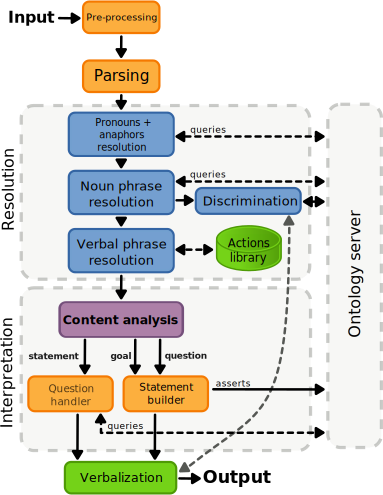
\includegraphics[width=0.6\linewidth]{images/dialogs/dialog_module_simple.pdf}
  \caption{The {\sc Dialogs} module has three main steps: the parsing,
  the interpretation and the verbalization. The interpretation module is
  responsible for both the \emph{resolution} and the semantic content
  \emph{analysis and translation}.} 
  \label{fig|dialog}
\end{figure}

As shown in Figure~\ref{fig|dialog}, the {\sc Dialogs} module is composed of
three main blocks. The user's input is first pre-processed. For instance,
\emph{I'm} constructs are expanded into \emph{I am} and then parsed. The parser
is a custom-made, rule-based (\ie grammar-free) tool that extracts the
grammatical structure from the user's sentence.

The result of the parsing is then sent to the \emph{interpretation} module, the
core of the approach.  Interpretation consists in three distinct operations:
the sentence \emph{resolution} (concepts grounding), the \emph{content
analysis} (what is the intent of the utterance: information, question or
desire) and the \emph{statement building} (translation into RDF statements).

The sentence resolution has three steps: {\it(1)} pronouns and anaphora are
replaced by, respectively, the correct speaker ID and the ID of the last object
spoken about (extracted from the dialogue history), {\it(2)} nominal groups are
disambiguated and grounded (noun phrase resolution), and {\it(3)} verbal groups
are resolved as well, and their associated thematic roles are retrieved (verbal
phrase resolution). Algorithm~\ref{algo|Resolution} describes the overall
process.  Next section describes specific examples to show how the noun and
verbal phrase resolution takes place.

\small
\begin{pseudocode}[ruled]{Resolution}{sentence, currentSpeaker}
\label{algo|Resolution}

\mathcal{G} \GETS \CALL{ParseNominalGroups}{sentence} \\

\FOREACH g \in \mathcal{G} \DO 
\BEGIN
   \mathcal{D} \GETS \CALL{GenerateDescription}{g} \STMTNUM{5.1em}{res.desc}\\
   candidates \GETS \CALL{Ontology.Find}{\mathcal{D}} \STMTNUM{4em}{res.onto}\\
   
   \IF \left|{candidates}\right| = 0 \THEN
    \BEGIN
      \OUTPUT{\mbox{Couldn't resolve the group!}} \\
      \EXIT \\
    \END
   \ELSEIF \left|{candidates}\right| = 1 \THEN
      id \GETS candidates[0] \STMTNUM{8em}{res.easy}\\

   \ELSE
      \BEGIN
	\IF \CALL{Ontology.CheckEquivalent}{candidates} \THEN
	  id \GETS candidates[0] \\
	\ELSE
	  id \GETS \CALL{Discrimination}{candidates} \\ %\STMTNUM{1em}{st.discrimination}\\
      \END \\
   \CALL{Replace}{g, id, sentence}
\END
\end{pseudocode}
\normalsize

As represented on Figure~\ref{fig|dialog}, interpretation tightly relies on the
communication with the knowledge base. All the concepts the robot manipulates
are stored in the \textit{ontology server} and retrieved through logical
queries, except for the verbs that are currently stored in a dedicated library
(the \emph{action library} on the diagram).

%%%%%%%%%%%%%%%%%%%%%%%%%%%%%%%%%%%%%
\section{Technical analysis}
\label{examples}

In order to better understand the overall process we next describe the
different steps based on three examples.

In this example, we assume some initial facts are present in the knowledge
base, both in the robot's \emph{own} model and in the \emph{human's} model.
Since the robot tries to ground a human utterance, all queries are sent 
to the \emph{human} model, \ie from the human perspective. 

\subsection{Informational content extraction}

Figure~\ref{dialog|ex1} shows a first example of human discourse grounding and
the extraction of informational content. We suppose that the robot knowledge
base only contains two initial statements in the human model. The user
asserts a new one: ``The yellow banana is big!''. 

\begin{figure}
    \centering
	\begin{tabular}{p{7cm}}
	\emph{Initial knowledge model of} \texttt{human\_01}\\
	\hline
    	\hspace{0.3cm}\stmt{banana\_01 \textbf{type} Banana} \\
    	\hspace{0.3cm}\stmt{banana\_01 \textbf{hasColor} yellow}\\
	
	\vspace{0.5em}
	\emph{Human input}\\
	\hline
	\hspace{0.3cm}``The yellow banana is big!'' \\

	\vspace{0.5em}
	\emph{Generated partial statements}\\
	\hline
	\hspace{0.3cm}\stmt{?obj \textbf{type} Banana} \\
    	\hspace{0.3cm}\stmt{?obj \textbf{hasColor} yellow} \\
    	\hspace{0.7cm}$\Rightarrow$ \stmt{?obj = banana\_01}\\

	\vspace{0.5em}
	\emph{Newly created statements}\\
	\hline
	\hspace{0.3cm}\stmt{banana\_01 \textbf{hasSize} big} \\
	\end{tabular}
\caption{First example of natural language grounding: the nominal group ``the
yellow banana'' is matched with the individual {\tt banana\_01}}.
\label{dialog|ex1}
\end{figure}


\small
\begin{pseudocode}[ruled]{GenerateDescription}{group}
\label{algo|GenerateDescription}

\PROCEDURE{GenerateDescription}{group} 
   noun \GETS \CALL{GetNoun}{group} \\ 
   \IF \CALL{Ontology.Lookup}{noun} \in (Instances) \STMTNUM{7.5em}{st.lookup} \THEN
   		\BEGIN
		id \GETS \CALL{Ontology.lookup}{noun}\\	
		\RETURN {\mathcal{D} + \{ *\ {\tt sameAs}\ <id> \}}\\
		\END
   \ELSE
    	\mathcal{D} = \mathcal{D} + \{ *\ {\tt type}\ <noun>\} \\
   
   \\
   det \GETS \CALL{GetDeterminant}{group} \\
   \IF det \in {\mbox(possessives)} \THEN
       \mathcal{D} = \mathcal{D} + \{ *\ {\tt isRelatedTo}\ <possessor>\} \\
    
    \IF det \in {\mbox(demonstratives)} \THEN
        \BEGIN
        \IF \CALL{Ontology.Check}{\{<currentSpeaker>\ {\tt focusesOn}\ *\}} \THEN 
            \mathcal{D} = \mathcal{D} + \{<currentSpeaker>\ {\tt focusesOn}\ *\}
        \ELSE
            \mathcal{D} = \mathcal{D} + \CALL{AnaphoricMatching}{} \STMTNUM{4em}{st.anaphoric} \\
        \END \\
   \\
   adjs \GETS \CALL{GetAdjectives}{group} \\
   \FOREACH adj \in adjs \DO
   	\BEGIN
   		\IF adj == <other> \THEN 
   			\BEGIN
   			id \GETS \CALL{History.GetMatchingGroup}{group} \STMTNUM{8em}{st.history}\\
   			\mathcal{D} = \mathcal{D} + \{ *\ {\tt differentFrom}\ <id> \}\\
   			\RETURN{D}\\
			\END   		
   		\ELSE
	     	\mathcal{D} = \mathcal{D} + \{ *\ {\tt hasFeature}\ <adj>\} \STMTNUM{9em}{st.adj} \\
    \END\\
    
   \\  
   nounComplements \GETS \CALL{GetNounComplements}{group} \\
   \FOREACH nouncmpl \in nounComplements \DO
     \mathcal{D} = \mathcal{D} + {\CALL{GenerateDescription}{nouncmpl}}\\
   
   
   \\  
   relativeClauses \GETS \CALL{GetSubordinateRelativeClauses}{group} \\
   \FOREACH relative \in relativeClauses \DO
   	\BEGIN
   	 \mathcal{G} \GETS \CALL{GetNominalGroups}{relative} \\
   	 \FOREACH g \in \mathcal{G} \DO
     	\mathcal{D} = \mathcal{D} + {\CALL{GenerateDescription}{g}}
    \END\\
     
   \\
   \RETURN{\mathcal{D}} 
\ENDPROCEDURE
\end{pseudocode}
\normalsize

\small
\begin{pseudocode}[ruled]{History.GetMatchingGroup}{group}
\label{algo|History}
\PROCEDURE{History.GetMatchingGroup}{group}
\COMMENT{Extract Nominal group from sentences stored in the history}\\
\mathcal{H} \GETS \CALL{History.GetAllNominalGoup}{}\\
\COMMENT{Generate description of the nominal group that is being processed.} \\
\COMMENT{The adjective  "other" is to be removed before calling this routine} \\
	\mathcal{G} \GETS \CALL{GenerateDescription}{group} \\ 
	
	candidates \GETS \mathcal{H} \cap \mathcal{G}\\
	\IF \left|{candidates}\right| = 0 \THEN
    \BEGIN
      \OUTPUT{\mbox{Couldn't find another object with the same characteristics!}} \\
      \EXIT \\
    \END
   \ELSEIF \left|{candidates}\right| = 1 \THEN
      id \GETS candidates[0]
   \ELSE
   	  id \GETS \CALL{Discrimination}{candidates}\\
   \RETURN{id}
\ENDPROCEDURE
\end{pseudocode}
\normalsize

We need to resolve the nominal group \emph{The yellow banana} to a known
concept.  A set of partial statements that describe the
concept is generated based on the grammatical parsing of the sentence
(algorithm~\ref{algo|GenerateDescription}). In the example, a banana
(\stmt{?obj \textbf{type} Banana}) that is yellow (\stmt{?obj \textbf{hasColor}
yellow})\footnote{Predicates like \concept{hasColor} or \concept{hasSize} that
bind \concept{banana\_01} to adjectives are extracted from a predefined
database of $[Predicate \rightarrow AdjectiveCategory]$, and falls back on the
generic \concept{hasFeature} predicate if the adjective is not known.}.  Based
on these partial statements a query is sent to the ontology server to retrieve
possible instances that match the description (algorithm~\ref{algo|Resolution},
\emph{(\ref{res.onto})}).

In this first simple case, the concept \concept{banana\_01} is unambiguously
matched (since there is only one possible banana) and returned. We can then add
the new information provided by the human, \ie the new statement
\stmt{banana\_01 \textbf{hasSize} big}, to the human model in the ontology
server.

\subsection{Intentional content through verb resolution}
The sentence in the first example is built with the state verb \emph{be} at
indicative. Let us examine a different example with an action verb at
imperative mode (\ie an order): ``Give me the banana". The process is
described in Figure~\ref{dialog|ex2}.

\begin{figure}
    \centering
	\begin{tabular}{p{7cm}}
	\emph{Initial knowledge model of} \texttt{human\_01}\\
	\hline
    	\hspace{0.3cm}\stmt{banana\_01 \textbf{type} Banana} \\
    	\hspace{0.3cm}\stmt{banana\_01 \textbf{hasColor} yellow}\\
	\end{tabular} \\

	\vspace{0.5em}

	\begin{tabular}{p{7cm}}
	\emph{Human input}\\
	\hline
    	\hspace{0.3cm}``Give me the banana.'' \\
	\end{tabular} \\

	\vspace{0.5em}

	\begin{tabular}{p{7cm}}
	\emph{Generated partial statements}\\
	\hline
    	\hspace{0.3cm}\stmt{?obj \textbf{type} Banana} \\
	\hspace{0.7cm}$\Rightarrow$ \stmt{?obj = banana\_01}\\

	\end{tabular} \\

	\vspace{0.5em}

	\begin{tabular}{p{7cm}}
	\emph{Newly created statements}\\
	\hline
    	\hspace{0.3cm}\stmt{human\_01 \textbf{desires} situation\_a3f74} \\
    	\hspace{0.3cm}\stmt{situation\_a3f74 \textbf{type} Give} \\
    	\hspace{0.3cm}\stmt{situation\_a3f74 \textbf{performedBy} myself} \\
    	\hspace{0.3cm}\stmt{situation\_a3f74 \textbf{actsOnObject} banana\_02} \\
    	\hspace{0.3cm}\stmt{situation\_a3f74 \textbf{receivedBy} human\_01} \\
	\end{tabular}

\caption{Second example: processing an order.}
\label{dialog|ex2}
\end{figure}

\label{processing_of_actions}

In order to capture the intentional content of a sentence (for example, an
order) we need to retain the semantics of the verb and its complements.
\emph{Thematic roles} allow to semantically link a verb to its complements.  We
use a small set of them that matches the relations the robot can actually
achieve. In this second example, the verb \emph{give} has three thematic roles:
\concept{performedBy}, \concept{actsOnObject} and \concept{receivedBy}.

The list of actions the robot can plan for (currently \emph{take},
\emph{place}, \emph{give}, \emph{show}, \emph{hide} and \emph{move}) along with
possible synonyms and their associated thematic roles are stored in a
predefined library of actions (Figure~\ref{fig|dialog}). For each action we identify and store the role
of the subject of the sentence --- always \concept{performedBy}; the role of
the direct object (for instance, \concept{actsOnObject}); and the role of each
of the indirect objects with their optional prepositions (for instance,
\concept{receivedBy})\footnote{Note that in example 2, ``give me the banana'',
the pronoun ``me'' appears before ``banana'', while it is an indirect
complement --- ``give it {\bf to me}''. The parser correctly handles these
cases.}. Moreover, we check with the help of the ontology that each holder of a
role has a consistent semantic. For instance, action \emph{Give} must have a
manipulable physical item (\emph{Artifact}) as direct object. Thus, if the
concept the robot finds for the thematic role \emph{actsOnObject} can not be
inferred to be an artifact, it goes back to the human saying it does not
understand.

Once the sentence is completely resolved and translated into a formal
representation (a human desire in this case\footnote{Orders are here
represented as human desires: the human desires a specific new situation.}), we
store it in the ontology server. The robot's decisional/executive layers should
then decide whether to execute the order or not. 

\subsection{Informational content extraction requiring clarification}
\begin{figure}
    \centering
	\begin{tabular}{p{7cm}}
	\emph{Initial knowledge model of} \texttt{human\_01}\\
	\hline
     	\hspace{0.3cm}\stmt{banana\_01 \textbf{type} Banana} \\
     	\hspace{0.3cm}\stmt{banana\_01 \textbf{hasColor} yellow} \\
     	\hspace{0.3cm}\stmt{banana\_02 \textbf{type} Banana} \\
     	\hspace{0.3cm}\stmt{banana\_02 \textbf{hasColor} green} \\
	\end{tabular} \\

	\vspace{0.5em}

	\begin{tabular}{p{7cm}}
	\emph{Human input}\\
	\hline
     	\hspace{0.3cm}``The banana is good.'' \\
	\end{tabular} \\

	\vspace{0.5em}

	\begin{tabular}{p{7cm}}
	\emph{Generated partial statements}\\
	\hline
     	\hspace{0.3cm}\stmt{?obj \textbf{type} Banana} \\
	\end{tabular} \\

	\vspace{0.5em}

	\begin{tabular}{p{7cm}}
	\emph{Robot output speech}\\
	\hline
     	\hspace{0.3cm}``The yellow one or the green one?'' \\
	\end{tabular} \\

	\vspace{0.5em}

	\begin{tabular}{p{7cm}}
	\emph{Human answer}\\
	\hline
     	\hspace{0.3cm}``The green one.'' \\
	\end{tabular} \\
    
	\vspace{0.5em}

	\begin{tabular}{p{7cm}}
	\emph{Newly created statements}\\
	\hline
     	\hspace{0.3cm}\stmt{banana\_02 \textbf{hasFeature} good} \\
	\end{tabular}

\caption{Ambiguity resolution: in this example, ``banana'' can refer to the
yellow banana (\concept{banana\_01}) or the green one (\concept{banana\_02}).
Discrimination routines handle the disambiguation process.} \label{dialog|ex3}
\end{figure}

This last example (Figure~\ref{dialog|ex3}) shows the resolution of ambiguous
concepts. In this case the user refers to ``the banana'' while two instances of
the \concept{Banana} class exist in the ontology. The robot needs to find out
to which instance the user is actually referring to. To this end,
disambiguation routines~\cite{Ros2010b} find differences between the instances
(in the example, one banana is yellow while the other one is green) and build a
sentence through the \emph{verbalization} module to ask the user a closed
question that will help clarify the ambiguity: ``Is it yellow or green?'' The
user's answer is parsed and added to the previous sentence. The resulting,
augmented, sentence (\ie ``Give me the green banana") goes again through all
the interpretation steps. This process is repeated until no ambiguities arise.
In the example, the \concept{banana\_02} is finally returned.

Several other strategies are used in parallel to disambiguate concepts without
having to ask for more information to the human: 

\begin{itemize}
	\item Which objects are currently visible to the human? If only one of
	them, then it is probably the one the user is talking about. 
	\item Did a previous interaction involved a specific object that would
	still be the subject of the current sentence?
	\item Is the user looking or pointing to a specific object?
\end{itemize}
 
While no examples involving questions have been detailled, \emph{W-} questions
and \emph{yes/no} questions can be processed in a similar way by
\textsc{Dialogs}. For instance, a question like: \emph{What is on the table?}
is grounded (to extract the relation \emph{isOn} and to find what \emph{table}
refers to) and transformed into the following kind of query: {\tt find ?var [?var isOn
table1]}.  Answers are converted back to a full sentence and uttered to the
human.


The next chapter (page~\pageref{chapter|evaluation}) presents several
experiments that make intensive use of the {\tt Dialogs} module.

\section{Planing for interaction}
\label{sect|planing-for-interaction}

\fxerror{TDB: dialogue + planing should allow the robot to answer questions
requiring temporal projection like: "Can you go to this place?"}


\chapter{Evaluation}
\label{chapter|evaluation}

\section{Comparison of oro-server with other existing systems}
\label{sect|evaluation-oroserver}

\section{Experimental evaluation}
\label{sect|experimental-evaluation}

\subsection{Experimental setup}
\label{sect|user-experiments}

\subsection{Simulation of HRI interaction}
\label{sect|simulation}


\subsection{User studies}
\label{sect|userstudies}



\chapter{Conclusion}
\label{chapter|conclusion}

\section{Scientific contributions}
\label{sect|scientific-contributions}

\section{Technical contributions}
\label{sect|technical-contributions}


%%%%%%%%%%%%%%%%%%%%%%%%%%%%%%%%%%%%%%%%%%%%%%%%%%%%%%%%%%%%%%%%%%%%%%%%%%%%%%%%%%%%%%%%%%%%%%%%%%%%%%%
%%%%%%%%%%%%%%%%%%%%%%%%%%%%%%%%%%%%%%%%%%%%%%%%%%%%%%%%%%%%%%%%%%%%%%%%%%%%%%%%%%%%%%%%%%%%%%%%%%%%%%%

\appendix
\appendixpage
\noappendicestocpagenum
\addappheadtotoc

% Adjustments headers
\fancyhead[RO, LE]{Appendix \thechapter --- \bfseries\leftmark}

\chapter{Description Logics Semantics}
\label{chapt|dl}

This appendix describes some notations and the naming convention of Description
Logics. The content of this page comes from the Wikipedia page on Descriptions
Logics\footnote{\url{http://en.wikipedia.org/wiki/Description_logic}} and the
DL Complexity Navigator~\cite{ZolinDLComplexityNavigator}. The academic reference
on this matter is~\cite{Baader2008}.


\paragraph{ACL} Let $N_C$, $N_R$ and $N_O$  be (respectively) sets of \emph{concept names}
(also known as \emph{atomic concepts}), \emph{role names} and \emph{individual
names} (also known as \emph{individuals}, \emph{nominals} or \emph{objects}).
Then the ordered triple ($N_C$, $N_R$, $N_O$ ) is the \emph{signature} of the
language.

Description Logics are implicitely \emph{Attributive Concept Language with
Complements}: $\mathcal{ALC}$.  The set of $\mathcal{ALC}$ \emph{concepts} is
the smallest set such that:

\begin{itemize}
    \item The following are \emph{concepts}:
    \begin{itemize}
        \item $\top$ (\emph{top} is a \emph{concept})
        \item $\bot$ (\emph{bottom} is a \emph{concept})
        \item Every $A \in N_C$ (all \emph{atomic concepts} are \emph{concepts})
    \end{itemize}

\item If $C$ and $D$ are \emph{concepts} and $R \in N_R$ then the following are \emph{concepts}:
        \begin{itemize}
            \item $C\sqcap D$ (the intersection of two \emph{concepts} is a \emph{concept})
            \item $C\sqcup D$ (the union of two \emph{concepts} is a \emph{concept})
            \item $\neg C$ (the complement of a \emph{concept} is a \emph{concept})
            \item $\forall R.C$ (the universal restriction of a \emph{concept} by a \emph{role} is a \emph{concept})
            \item $\exists R.C$ (the existential restriction of a \emph{concept} by a \emph{role} is a \emph{concept})
        \end{itemize}

\end{itemize}

 %% The following definitions follow the treatment in Baader et al.<ref name="DLHB"/>
 %% 
 %% A \emph{terminological interpretation} $\mathcal{I}=(\Delta^{\mathcal{I}},
 %% \cdot^{\mathcal{I}})$ over a \emph{signature} $(N_C,N_R,N_O)$ consists of
 %% 
 %% \begin{itemize}
 %%     \item a non-empty set $\Delta^{\mathcal{I}}$ called the \emph{domain}
 %%     \item a \emph{interpretation function} $\cdot^{\mathcal{I}}$ that maps:
 %%         \begin{itemize}
 %%         \item every \emph{individual} $a$ to an element $a^{\mathcal{I}} \in \Delta^{\mathcal{I}}$
 %%         \item every \emph{concept} to a subset of $\Delta^{\mathcal{I}}$
 %%         \item every \emph{role name} to a subset of $\Delta^{\mathcal{I}}  \times \Delta^{\mathcal{I}}$
 %%         \end{itemize}
 %% \end{itemize}
 %% 
 %% such that
 %% 
 %% \begin{itemize}
 %%     \item $\top^{\mathcal{I}} = \Delta^{\mathcal{I}}$
 %%     \item $\bot^{\mathcal{I}} = \emptyset$
 %%     \item $(C \sqcup D)^{\mathcal{I}} = C^{\mathcal{I}} \cup D^{\mathcal{I}}$ \emph{(union means disjunction)}
 %%     \item $(C \sqcap D)^{\mathcal{I}} = C^{\mathcal{I}} \cap D^{\mathcal{I}}$ \emph{(intersection means conjunction)}
 %%     \item $(\neg C)^{\mathcal{I}} = \Delta^{\mathcal{I}} \setminus C^{\mathcal{I}} $ \emph{(complement means negation)}
 %%     \item $(\forall R.C)^{\mathcal{I}} = \{x \in \Delta^{\mathcal{I}} | \texttt{for} \; \texttt{every} \; y, (x,y) \in R^{\mathcal{I}} \;  \texttt{implies} \; y \in C^{\mathcal{I}} \} $
 %%     \item $(\exists R.C)^{\mathcal{I}} = \{x \in \Delta^{\mathcal{I}} | \texttt{there} \; \texttt{exists} \; y, (x,y) \in R^{\mathcal{I}} \; \texttt{and} \; y \in C^{\mathcal{I}}\} $
 %% 
 %% \end{itemize}
 %% 
 %% Define $\mathcal{I} \models$ (read \emph{I models}) as follows
 %% 
 %% \paragraph{TBox}
 %% 
 %% \begin{itemize}
 %%     \item $\mathcal{I} \models C \sqsubseteq D$ if and only if $C^{\mathcal{I}} \subseteq D^{\mathcal{I}}$
 %%     \item $\mathcal{I} \models \mathcal{T}$ if and only if $\mathcal{I} \models t$ for every $t \in \mathcal{T}$
 %% 
 %% \end{itemize}
 %% 
 %% \paragraph{ABox}
 %% 
 %% \begin{itemize}
 %%     \item $\mathcal{I} \models a : C$ if and only if $a^{\mathcal{I}} \in C^{\mathcal{I}}$
 %%     \item $\mathcal{I} \models (a,b) : R$ if and only if $(a^{\mathcal{I}},b^{\mathcal{I}}) \in R^{\mathcal{I}}$
 %%     \item $\mathcal{I} \models \mathcal{A}$ if and only if $\mathcal{I} \models a$ for every $a \in \mathcal{A}$
 %% 
 %% \end{itemize}
 %% 

This can be formulated as ACL languages allowing:
\begin{itemize}
    \item Atomic negation (negation of concept names that do not appear on the left hand side of axioms)
    \item Concept intersection
    \item Universal restrictions
    \item Limited existential quantification
\end{itemize}

The expressiveness of ACL languages can be extended, following this naming convention:

\begin{itemize}
    \item $\mathcal{F}$ for support of functional properties,

    \item $\mathcal{N}$ for cardinality restrictions
    (\concept{owl:cardinality}, \concept{owl:maxCardinality}, implies
    $\mathcal{F}$),

    \item $\mathcal{Q}$ for qualified cardinality restrictions (available in
    OWL 2, cardinality restrictions that have fillers other than
    \concept{owl:Thing}, implies $\mathcal{N}$), 

    \item $\mathcal{E}$ for full existential qualification (Existential
    restrictions that have fillers other than \concept{owl:Thing}),

    \item $\mathcal{U}$ for concept union,

    \item $\mathcal{C}$ for complex concept negation,

    \item $\mathcal{S}$ for role transitivity,

    \item $\mathcal{H}$ for role hierarchy (subproperties -
    \concept{rdfs:subPropertyOf}),

    \item $\mathcal{R}$ for complex role inclusion axioms (reflexivity and
    irreflexivity; role disjointness, implies $\mathcal{S}$ and $\mathcal{H}$),

    \item $\mathcal{O}$ for nominals (enumerated classes of object value
    restrictions - \concept{owl:oneOf}, \concept{owl:hasValue}),

    \item $\mathcal{I}$ for inverse properties,

    \item $\mathcal{(D)}$ for use of datatype properties, data values or data
    types.

\end{itemize}

OWL2 is a $\mathcal{SROIQ(D)}$ languages, which can be written in expansed form
as $\mathcal{ALC} + \mathcal{SHRFNQOI(D)}$. This is the expressiveness level of
the ORO common-sense ontology.




\chapter{Task representation in the ontology}
\label{appendix|tasks}

\emph{First warning}: I'm talking here only of {\bf task} representation in
robotics. Plans are another matter.

\emph{Second warning}: the current approach for extending the ontology is to
rely as much as possible on OpenCyc \footnote{OpenCyc online search:
\href{http://sw.opencyc.org/}{http://sw.opencyc.org/}} (I will prefix all
OpenCyc concept with {\tt cyc:\ldots{}}). If a concept or a predicate needed in
the robotics context does not exist in OpenCyc, then we can create it in our
own namespace (I'll prefix these proposed concepts with {\tt rcs:\ldots{}} for
RoboticsCommonSense).

\emph{Third warning}: There is few (5) references at the very end of this page.
Please let me know if you have other papers related to task modelling in
ontologies!


\section{What are tasks for the ontology?}

Before looking at what tasks are, let think for a second why we would want to
represent them at all in the ontology.

Usually, managing plans and tasks in a robot involve these kind of cognitive
capacities:


\begin{enumerate}

\item  the ability to infer which tasks could be started at any time,

\item  the ability to check that if we do some task, it won't bring the world
in an inconsistent state,

\item  more generally, the ability to predict the state of the world after some
task execution,

\item  retrieve tasks that should be started to achieve some result,

\item  knowing how long a task lasts.

\item  \ldots{}[what else?]

\end{enumerate}

Most of these capabilities are bound to complex reasoning systems
(\ldots{}planners!), that must take into account very different things (like
time, current activity, agent's desires\ldots{}) to select tasks and build
plans.

The ontology, as built by the robot during its lifetime, is a model of the
world that can help the planner.

It efficiently represents some of the knowledge required for planning and task
execution:


\begin{itemize}

\item  Agents state (like, busy, reading, standing, talking\ldots{}), desires
(short or long term goals)

\item  Agents capacities (technically doable actions)

\item  Physical world state (location of objects,\ldots{})

\item  Common sense knowledge (role, usage of objects\ldots{})

\end{itemize}

Note that this knowledge is mostly declarative. Storing of procedural knowledge
is more difficult. But we'll come to it later.

Now, what are \emph{tasks}, from the ontology point of view?


\begin{enumerate}

\item  Tasks are {\bf instances} of {\bf actions} that have some purpose. As
it, they are instances of {\tt cyc:PurposefulAction}

\item  The type of action can be further refined by using sub-classes of
PurposefulAction (like {\tt cyc:Movement-TranslationEvent}, {\tt
cyc:Reading}\ldots{} the robot is expected to provide - likely at startup - the
list of actions it can achieve depending on its hardware)

\item  a {\tt cyc:PurposefulAction} is {\tt cyc:performedBy} one (or several)
{\tt cyc:EmbodiedAgent}.

\end{enumerate}

\section{Different facets of the reality}

Now, let's enter in the difficult part:

A task may have a specific context as prerequisites or on the contrary, may
imply some new state of the world as post-condition.  Since these two aspects
are largely symmetric, I will only discuss post-conditions.

Post-conditions are difficult to represent, because the new state of the world
they represent may contradict with the current state, thus leading to
inconsistencies.

Let's take an example. Imagine the task: \emph{"cracking an egg"}. To build a
model of this task, we need somehow to encode the post condition: {\tt the egg
shell is broken} [stmt1].

We can as well assume that the state of the egg shell before we crack it is:
{\tt the egg shell is not broken} [stmt2].

If we add both these statements {\tt [stmt1]} and {\tt [stmt2]} in the ontology
(ie, we assert them), the ontology becomes inconsistent, and no reasoning is
possible.

For people doing planning, there's no real issue there: that's precisely the
planner role to {\bf replace} {\tt [stmt2]} by {\tt [stmt1]} when the task is
achieved. In this case, the two statements wouldn't \emph{hold} (ie, be
asserted to be true) at the same time, and everything remains consistent.

OpenCyc has another, very powerful way to deal with different "truths" of this
kind: {\bf micro-theories}. Within a microtheory, a certain set of facts must
hold. But not necessary outside. To put it in another way, OpenCyc doesn't
generally requires the set of facts to be consistent. Only facts asserted in a
specific microtheory must be consistent with each others.

In the egg example, it means that statements 1 and 2 can be asserted at the
same time. Two microtheories must be created as well (called {\tt
cyc:TaskState} in this case), one that would describe the world {\bf before}
the task \emph{"cracking an egg"} (it would be linked to the task by the {\tt
cyc:taskPrerequisites} predicate), one that would describe the world {\bf
after} the task completion (linked with {\tt cyc:taskToAchieve} predicate).

So far, so good.

The problem is: such a "microtheory"-based approach doesn't belong to the
Description Logics (it's not anymore a first order logic system), and thus
considerably reduce the practical inference capabilities.

Second problem (that is partially a consequence of the first one): OWL, the
widely-used ontology format we are using, has no notion of microtheory, neither
have most of the semantic tools like Protege, OWL-API\footnote{Application
Programming Interface}, Jena or Pellet.


\section{A simple case: the Move task}

So in practice, some mitigation must be done.

Since the semantics behind {\tt cyc:TaskState}, {\tt cyc:RealizedTaskState} (an
effective, realised state of the world), {\tt cyc:taskPrerequisites}, {\tt
cyc:taskToAchieve} and {\tt cyc:taskConstraints} (that expresses specific
constraints applied during task execution) is still relevant to us, the
question is: how to build {\tt cyc:TaskState} without {\tt cyc:Microtheory}?

Let's have a look to a simple yet "real world" example, extracted from the
LAAS' HATP planner task model:



\begin{alltt}

action Move(Agent ag1, Place p1, Place p2)
 {
   preconditions
   {
     p1 != p2;
     ag1.posTopo == p1;
   };

   effects
   { ag1.posTopo == p2; };
 } 

\end{alltt}

Pre- and post-conditions and the relations between entities (ag1, p1, p2) are
easy to understand from this model.

How to represent it in the ontology?

Let's start with the pre-condition {\tt P1 != P2}. We want to create a new kind
of {\tt cyc:TaskState} that says: "Two locations are different".

Mathematically speaking: $ \exists x,y \in Location / x \neq y$. OWL speaking:



\begin{alltt}

//This class would mean: all locations that are attached with rcs:forLocation predicate must be
different from each other.
rcs:DifferentLocationState subClassOf cyc:TaskState
rcs:forLocation hasDomain rcs:DifferentLocationState
rcs:forLocation hasRange cyc:SpatialThing-Localized

//One instance:
precondition1 rdf:type rcs:DifferentLocationState
precondition1 forLocation p1
precondition1 forLocation p2

\end{alltt}

Same thing for an rcs:IdenticalLocationState:



\begin{alltt}

rcs:IdenticalLocationState subClassOf cyc:TaskState
rcs:forLocation hasDomain rcs:IdenticalLocationState

//Two instances:
precondition2 rdf:type rcs:IdenticalLocationState
precondition2 forLocation ag1
precondition2 forLocation p1

postcondition1 rdf:type rcs:IdenticalLocationState
postcondition1 forLocation ag1
postcondition1 forLocation p2

\end{alltt}

Then we can define the task itself:



\begin{alltt}

//Abstract model of the task
laas:Move subClassOf cyc:Movement-TranslationEvent

laas:Move subClassOf (cyc:taskPrerequisites some IdenticalLocationState)
laas:Move subClassOf (cyc:taskPrerequisites some DifferentLocationState)

laas:Move subClassOf (cyc:taskToAchieve some IdenticalLocationState)

//Instanciation:
move1 type laas:Move
move1 performedBy ag1
move1 fromLocation p1
move1 toLocation p2
move1 taskPrerequisites precondition1
move1 taskPrerequisites precondition2
move1 taskToAchieve postcondition1

\end{alltt}

Two big issues there:


\begin{itemize}

\item  DifferentLocationState/IdenticalLocationState conditions, as formalized
above, lack expressivity: we, as robot designers, "decide" that
"DifferentLocationState" means that the locations must be disjoint, but there
no way to actually this rule is actually enforced when reasoning. The only
explicit constraint is that DifferentLocationState or IdenticalLocationState
involve locations (instances of {\tt cyc:SpatialThing-Localized}). But we don't
formally say that these locations must be disjoint or identical.

\item  The abstract model of the task doesn't maintain the semantic: it merely
says that a "Move" task must have 2 preconditions, one of kind "different
location", one of kind "identical location" and 1 post-condition of type
"identical location". But the fact that explicitly the location {\tt p1} and
{\tt p2} must be different (and not, for instance, {\tt ag1} and {\tt p1} or
even {\tt the moon} and {\tt the sun}) is not kept. We get it back at
instanciation time, but it seriously reduces the relevance of such a task
description for anything useful.

\end{itemize}

As it, it's difficult to me to see the relevance of such a task model for
robotics. The original task model from HATP is ways simpler and easier to read.
But let dig a bit futher.


\section{Fluent-based approach}

The current TUM approach is based on fluents \footnote{A fluent is a condition
that can change truth value over time, cf
\url{http://en.wikipedia.org/wiki/Fluent_artificial_intelligence}} and events.

The idea is to represent the various states of the world with instances of {\tt
rcs:Holds} and {\tt rcs:Occurs} classes, associated to a fluent and a time (or
time interval).

Some of the fluents they use:


\begin{itemize}
\item  contains(obj, container)
\item  supports(obj, support)
\item  attached(obj1, obj2)
\item  \ldots{}
\end{itemize}
If we take the egg example:

{\tt occurs(breaking(egg), 10.2)} (which means that the egg was broken at time
10.2s) would be represented in the ontology as:



\begin{alltt}

event231 rdf:type cyc:BreakingEvent
event231 hasObject egg

state746 rdf:type tum:Occurs
state746 fluent event231
state746 occursAt 10.2

\end{alltt}

or, for situations, {\tt holds(broken(egg), [10.3, +INF])} (which formally
mean: from time 10.3 until +INF, the statement "the egg is broken" holds) would
become:



\begin{alltt}

fluent471 rdf:type tum:BrokenFluent
fluent471 hasSubject egg

state746 rdf:type tum:Holds
state746 fluent fluent471
state746 startsAt 10.3
state746 finishsAt +INF

\end{alltt}

This representation matches situation calculus (or variants like event/fluent
calculus) theories [McCarty1969] and takes explicitly into account the time
(either time points or time intervals).

I don't know well enough temporal reasoning and temporal planning to have any
insight regarding the relevance of such a model, but it seem potentially very
powerful to represent plans because of the tight coupling with time.

However, since the causal relations are somehow lost, I don't see how it could
be used to create a plan.

Another issue is the lack of integration with classical first-order logic
reasoners: fluents are a kind of statement reification and limit the ability of
reasoner to further infer the new state of the world after the conclusion of
some action. To put it another way: when a fluent holds, we can not directly
infer the consequences of this fluent. Even if the fluent {\tt BrokenEgg}
holds, the statement {\tt egg rdf:type cyc:Fractured} is not asserted anyhow,
and we couldn't directly query the ontology for "the list of broken objects"
for instance.

In any case, I would need more input on fluent-based representations.


\section{Introducing rules}

To issue of low expressivity we had with tasks represented as pure OWL
statement can be improved with rules. The example below, written in
SWRL\footnote{While not an introduction, a very valuable resource on SWRL is
the Protege FAQ \url{http://protege.cim3.net/cgi-bin/wiki.pl?SWRLLanguageFAQ}},
is the formalisation of the conditions for {\tt IdenticalLocationState} to be
true:



\begin{alltt}

IdenticalLocationState(?state) \(\land\)
forLocation(?state, ?p1) \(\land\)
forLocation(?state, ?p2) \(\land\)
sameAs(?p1, ?p2)
\(\Rightarrow\) RealizedTaskState(?state)

\end{alltt}

Same thing for {\tt DifferentLocationState}:



\begin{alltt}

DifferentLocationState(?state) \(\land\)
forLocation(?state, ?p1) \(\land\)
forLocation(?state, ?p2) \(\land\)
differentFrom(?p1, ?p2)
\(\Rightarrow\) RealizedTaskState(?state)

\end{alltt}

Let create a new class, {\tt rcs:UndertakeableAction}, that hold all the action
whose pre-conditions are satisfied. We can complete the example:



\begin{alltt}

//Define our variables
EmbodiedAgent(?ag1) \(\land\)
SpatialThing-Localized(?p1) \(\land\)
SpatialThing-Localized(?p2) \(\land\)

//Bind the Move action
Move(?action) \(\land\)
performedBy(?action, ?ag1) \(\land\)
fromLocation(?action, ?p1) \(\land\)
toLocation(?action, ?p2) \(\land\)

//Bind the agent position
hasLocation(?ag1, ?p3) \(\land\)

//Check precondition 1
DifferentLocationState(?precondition1) \(\land\)
forLocation(?precondition1, ?p1) \(\land\)
forLocation(?precondition1, ?p2) \(\land\)
RealizedTaskState(?precondition1) \(\land\)

//Check precondition 2
IdenticalLocationState(?precondition2) \(\land\)
forLocation(?precondition2, ?p1) \(\land\)
forLocation(?precondition2, ?p3) \(\land\)
RealizedTaskState(?precondition2)

\(\Rightarrow\) UndertakeableAction(?action)

\end{alltt}

This rule would be triggered by the reasoner if and only if:


\begin{enumerate}

\item  At least one agent is asserted or inferred (it is bound to {\tt ?ag1}),

\item  Two other, different locations have been asserted of inferred ({\tt ?p1}
and {\tt ?p2})\footnote{Since OWL and SWRL use the Open World Assumption, it
means that {\tt ?p1} and {\tt ?p2} must be {\bf explicitly} disjoint}

\item  At least on instance of the action {\tt Move} exists ({\tt ?action}),
performed by {\tt ?ag1} from {\tt ?p1} to {\tt ?p2}.

\item  {\tt ?p3} will be successively bound to every current location of {\tt
?ag1}

\item  One instance of a {\tt DifferentLocationState} context exists with {\tt
?p1} and {\tt ?p2} as locations. This context is a \emph{realised context}.

\item  Symmetrically, one instance of a {\tt IdenticalLocationState} context
exists with {\tt ?p1} and {\tt ?p3} as locations. This context is a
\emph{realised} as well.

\end{enumerate}

If all these conditions hold, then the {\tt ?action} is an {\tt
UndertakeableAction}.

{\bf Three important remarks:}


\begin{itemize}
\item  One could suggest to \emph{factor} the code with a rule that would say:
"For any Action, if all pre-conditions are RealizedState, then the action is
undertakeable". Somethink like:


\begin{alltt}

Move(?action) \(\land\)
taskPrerequisites(?action, ?state) \(\land\)
RealizedState(?state)
\(\Rightarrow\) UndertakeableAction(?action)

\end{alltt}

It's simply not possible in OWL because of the Open World Assumption (OWA):
there is not way to be certain that {\bf all} states are realised because there
is no way to know {\bf all} the prerequisite states. The idea is something
like: "it's not because I don't know it - ie, it is not asserted - that it
doesn't exist".


\item  For post-conditions, it's important to understand that we {\bf cannot}
\emph{apply} the result of a rule to the ontology.

What does it mean? It means that something like that:



\begin{alltt}

Move(?action) \(\land\)
SuccessfullyCompleteAction(?action) \(\land\)
IdenticalLocationState(?postcondition1) \(\land\)
forLocation(?postcondition1, ?p2) \(\land\)
forLocation(?postcondition1, ?p3) \(\land\)
\(\Rightarrow\) RealizedState(?postcondition1)

\end{alltt}

or even simpler:



\begin{alltt}

Move(?action) \(\land\)
SuccessfullyCompleteAction(?action) \(\land\)
fromLocation(?action, ?p1) \(\land\)
toLocation(?action, ?p2)
\(\Rightarrow\) sameAs(?p1, ?p2)

\end{alltt}

will work, but only as long as the action is considered a {\tt
SuccessfullyCompleteAction}. It means as well that if we do another movement
({\tt move2}) but {\tt move1} is still a {\tt SuccessfullyCompleteAction}, then
we are likely to have an inconsistency (or unwanted inferences): the robot will
be at several places at the same time.

And even if we can \emph{add} somehow new statements, we can not \emph{remove}
statement because of the monotonic paradigm of OWL\footnote{About monotonicity
and non-monotonicity, cf Wikipedia:
\url{http://en.wikipedia.org/wiki/Monotonicity_of_entailment}. About
non-monotonic reasoning, cf also
\url{http://www.aaai.org/AITopics/pmwiki/pmwiki.php/AITopics/Nonmonotonicity}}.
It's not possible for instance to complete the post-condition rule to say that
the agent is not anymore in {\tt p1}.


\item  Finally, one could conversely want to use post-condition with rules to
know if an action was successful:


\begin{alltt}

Move(?action) \(\land\)
performedBy(?action, ?ag1) \(\land\)
hasLocation(?ag1, ?p1) \(\land\)
toLocation(?action, ?p2) \(\land\)
sameAs(?p1, ?p2)
\(\Rightarrow\) SuccessfullyCompleteAction(?action)

\end{alltt}

It's doesn't prove that the action was successful - or did even occurred at
all. It only says that the world is in a state that match the post-conditions
of the action {\tt Move}. But this remark is not specific to rule reasoning.

\end{itemize}

At the end, what should we think of rule-based representations of pre- and
post-conditions? I'll come back to this question in the conclusion, but for
now, it's important to underline the relative complexity of correctly writing
SWRL rules in the Description Logics safe space. It can however prove useful to
check that the world state is a context that permit some actions to occur or
conversely that matches the expected outcome of some other actions.


\section{Drawing a conclusion}

Our original questions where:

\begin{enumerate}

\item  How to express \emph{pre- and post-conditions} in the ontology? and how
the knowledge processing framework could be used to check or enforce them?

\item  What \emph{abstract model} of a task could be formalized in the
ontology?

\item  How could we rely on the ontology to \emph{instantiate} tasks?

\end{enumerate}

In order to reach some conclusion on these complementary perspectives, we
should go back to the "big picture" behind task planning. Let's consider a
simple scenario that would instatiate the {\tt Move} task in a real case:

\emph{A human and a robot are face to face, at breakfast table. The human ask
the robot to bring on cereals.}

If nothing special prevents the robot to go to the cupboard, it has two moves
to plan: from the table to the cupboard and back from the cupboard to the
table.

What is the process involved? Roughly:


\begin{enumerate}

\item  We first need to convert the human order from natural language to a
machine processable representation: something like {\tt human desires cereals}.

\item  Some supervision module receive this order, do an initial grounding
(\emph{which human? what are cereals? which cereal box do I know?}), add a new
goal

\item  The supervision ask the task planner to generate a plan to {\tt bring
cereal\_instance1 to human\_instance1}

\item  the task planner retrieves some more infos (like the location of the
instances involved) and proposes a list of (instanciated) tasks to the
supervision.

\item  the supervision decides to start (or not) the execution of the plan,
starts individual tasks and monitor the global unwinding of the plan.

\end{enumerate}

\subsection{Task instanciation}

So, how can the ontology-based knowledge base help in this process?


\begin{itemize}

\item  Obviously by providing common references to objects, agents, locations.

\item  By storing informations related to the concepts (location of an agent,
of an object). Further, this knowledge can be uniformly accessed, be it
originally provided by the robot own perception or external datastores (for
instance web-based).

\item  These references along with inference capabilities can be a corner stone
for the grounding requirements mandated by supervision or planning.

\end{itemize}

These three aspects are most useful for {\bf task instanciation}, are well
understood, a already largely implemented. Task representation can and should
benefit of the symbolic framework offered by ontologies.


\subsection{Pre- and post-conditions}

Then, on the reasoning side, can our knowledge processing tool help with
dealing with pre- and post-condition? Or, are ontologies and associated
reasoning tool relevant for the \emph{legality task} (are tasks performable?)
and the \emph{temporal projection task} (what will be the state of the world
after some tasks are performed?), as called by Levesque [Levesque2007]? (he
notes by the way that, based on situation calculus and assuming we have access
to tasks preconditions, the \emph{legality task} can be reduced to the
\emph{projection task}).

We have seen that standard OWL semantics doesn't allow for a satisfying way to
represent the complex semantic and logic of pre- and post-conditions, even in
simple case like the {\tt Move} action.

However, the rule-based approach allows us to effectively represent the full
expressivity of these constraints. Since rule language like SWRL are actually
implemented in current reasoners like Pellet, such description of task
conditions could be actually suitable for checking both that:


\begin{itemize}

\item  the robot believes the current world state allows a given action to take
place,

\item  the robot believes that it reached a state where the intended results of
an actions are realised (which may mean that either the action was successfully
complete or that some environment changes lead to an equivalent state of the
world)

\end{itemize}

\emph{Per se} this knowledge is useful for the supervision. But it can not
replace the need for the planer to reason itself on pre- and post-conditions
since the reasoning that the ontology framework provides applies only to the
{\bf current} state of the world. Indeed, traditional first-order logic
reasoners don't offer, as far as I know, to build hypothetical world models
that would come out of some actions (in part because of the monotonic reasoning
paradigm). This would be necessary to predict future state of the world, as
required for planning. The fluent paradigm associated to a dedicated reasoner
could however provide a mean to reason in the future.

Moreover, as we already stated, using such rules for post-condition only allows
to check if the post-conditions are met. It doesn't prove that the action was
achieved. {\bf More importantly}, none of the various solutions we presented
above allow to \emph{apply} post-conditions to the ontology. An external module
(likely the supervisor) must take care of updating the ontology according to
the consequences of the action, adding new statements and removing deprecated
facts. Note however that in many cases these changes are made "on-line", in
parallel to the action execution (in the example of the human and cereals, we
can assume for instance that some localization module will update the position
of the robot in the ontology as soon as the robot move).

At the end of the day, it seems to me that representing certain \emph{states of
the world} as a set of constraints expressed as rules can be relevant. It would
allow the robot to be \emph{conscious} that a specific situation occurs. But,
to be useful, these {\tt cyc:TaskState} or contexts must be easy to create "on
the fly" by the planner or by the supervisor, either to describe a context
required by a new task or on the contrary to express an expected situation. It
could be useful to develop to this end a library dedicated to SWRL content
generation.


\subsection{Task abstract model}

Last aspect: are abstract models of tasks easily and effectively representable
in our current, OWL-based, knowledge frameworks?

Brandon Ibach, on the pellet-user list, summarize the model of the {\tt Move}
task this way (well, just the "precondition" part):

\begin{alltt}

Place
Agent [ hasPosition(Place) ]
Action
    UndertakableAction \(\leftarrow\) EligibleMove \(\land\) NonEmptyMove
    Move [ hasAgent(Agent) hasFrom(Place) hasTo(Place) ]
        EligibleMove \(\leftarrow\) Move(m) \(\land\) hasAgent(m, a) \(\land\) hasPosition(a, p) \(\land\) hasFrom(m, f) \(\land\)
sameAs(p, f)
        NonEmptyMove \(\leftarrow\) Move(m) \(\land\) hasFrom(m, f) \(\land\) hasTo(m, t) \(\land\) differentFrom(f, t)

\end{alltt}

This can be probably considered as an abstract model of the task. This model
mixes pure OWL statements with SWRL extensions. It's formally sound, but I
doubt of the practical usability for the planner. Maybe the people from
planning could precise a bit how they would like to use this kind of abstract
model (as storage for the list of possible tasks, for instance?)


\section{Some previous work \& references}


\begin{itemize}

\item  {\bf [McCarthy1969]
\url{http://centria.di.fct.unl.pt/~jja/agregacao/teaching/assets/paginasCadeiras/rcr/docs/actionPapers/mcchay69.pdf}:
Some philosophical problems from the standpoint of artificial intelligence -
\emph{J. McCarthy, P. Hayes - 1969}} This major paper states the issue of How
it "can be proved that a strategy will achieve a goal". McCarthy introduces
there the \emph{situation calculus}.

\item  {\bf [Artale1999]
\url{http://citeseerx.ist.psu.edu/viewdoc/download?doi=10.1.1.25.1319&rep=rep1&type=pdf}
Representing a robotic domain using temporal description logics, \emph{A
Artale, E Franconi - AI EDAM, 1999}}

\item  {\bf [Gil2005]
\url{http://ftp.isi.edu/~gil/papers/AImag05.pdf} Description Logics and
Planning, \emph{Y. Gil - AI Magazine, 2005}}, A survey of previous work on
combining planning techniques with expressive representations of knowledge in
description logics to reason about tasks, plans, and goals.

\item  {\bf [Levesque2007]
\url{http://www-kbsg.informatik.rwth-aachen.de/system/files/CogRobKRHandbook.pdf}
Cognitive robotics, \emph{ H. Levesque and G. Lakemeyer, in Chapter 24 in
Handbook of Knowledge Representation, Elsevier, 2007 }}

\item  {\bf [Clark2009]
\url{http://clarkparsia.com/weblog/2009/02/04/what-is-automated-planning/} 
What is automated planning?, \emph{K. Clark - 2009}}, from the creator of the
Pellet reasonner. They use an HTN planner with a task representation based on
\url{http://en.wikipedia.org/wiki/OWL-S} OWL-S

\end{itemize}


\chapter{The \emph{Knowledge API}}
\label{chapter|kb-api}

Refer to section~\ref{sect|knowledge-api} for the rationale of the API, as well
as a discussion of its limitations.

\section{Conventions}

\begin{itemize}

    \item  \textbf{Service}: we call \emph{service} the set of all methods
    defined by this API.

    \item  \textbf{Method}: \emph{method} refers to one single remote function
    offered by the service. The terms function, method, and procedure can be
    assumed to be interchangeable.

    \item  The \textbf{Service provider} or \textbf{implementation} is a
    software that implement the API.

    \item  A \textbf{policy} is a (extensible) set of rules that defines in
    which ways the knowledge must be altered. It is represented as a dictionary
    of (keys, values). The section~\ref{sect|kbapi-policies} details the
    content of these policies.

\end{itemize}

\section{Statements, partial statements and rules}


\subsection{Resources and literals}


All entities in the knowledge base are either \textbf{resources} or
\textbf{literals}. Resources can be classes, predicates or instances.

Resources (\ie, not literals) must start with a letter and can be comprised of
symbols [{\tt a-zA-Z0-9\_}].

They may be prefixed with a namespace prefix (like in \texttt{rdf:type}) or
come with a complete namespace URI (like
\texttt{$<$\href{http://www.w3.org/1999/02/22-rdf-syntax-ns\#type}{http://www.w3.org/1999/02/22-rdf-syntax-ns{\textbackslash}\#type}$>$}).
In this case, the full URI (the namespace and the resource name) must be
enclosed between $<$ and $>$. If no namespace is provided, it is assumed to be
defined in the server default namespace.

Literals should follow the SPARQL syntax for
literals\footnote{\url{http://www.w3.org/TR/rdf-sparql-query/\#QSynLiterals}}.
Give give below some examples of valid literals:

\begin{itemize}

    \item  The boolean {\bf true} can be represented either as
    \texttt{"true"\^{ }\^{ }xsd:boolean} or as \texttt{true},

    \item  The integer {\bf 123} can be represented either as \texttt{123\^{
    }\^{ }xsd:int} or as \texttt{123}. \texttt{"123"\^{ }\^{ }xsd:int} is also
    acceptable.

    \item  The double {\bf 1.23} can be represented either as \texttt{1.23\^{
    }\^{ }xsd:double} or as \texttt{1.23}. \texttt{"1.23"\^{ }\^{ }xsd:double}
    is also acceptable.

    \item  Strings are either single or double quoted: \texttt{"Hello Word"},
    \texttt{'Hello Word}', \texttt{"Hello Word"\^{ }\^{ }xsd:string} all
    describe the same literal.

    \item  User-defined dataypes can be represented with \texttt{"xyz"\^{ }\^{
    }$<$\href{http://example.org/ns/userDatatype}{http://example.org/ns/userDatatype}$>$}
    or \texttt{"xyz"\^{ }\^{ }ns:userDatatype}.

\end{itemize}

\subsection{Statements}


\paragraph{General syntax}

Two syntaxes are admissible to represent a \textbf{statement} (or
\textbf{axiom}).  The general one is a string starting with a predicate
\texttt{p} followed by a set in brackets of comma-separated arguments:

    \begin{center} \tt p(a1, ..., an) \end{center}

where \texttt{n} is the arity of the predicate. For instance:

    \begin{center}  \tt cutsWith(human0, bred0, knife0) \end{center}

The predicate must be a resource, as well as at least one of the arguments.
Other arguments may be either resources or literals.

\paragraph{Infix syntax}

As a special case, the infix syntax (\emph{subject predicate object}) is
acceptable for binary predicates (in this case without commas or brackets):

    \begin{center} \tt s p o \end{center}

For instance:

    \begin{center} \tt sky0 hasColor blue \end{center}


Further examples include:

\begin{itemize}
    \item {\tt Age(EiffelTower, 300)},

    \item {\tt filledWith(my\_cup, coffee)}, which is strictly equivalent to
    {\tt my\_cup filledWith coffee},

    \item {\tt my\_cup rdf:type opencyc:Cup},

    \item {\tt my\_cup weights 10.5} (assuming that the {\tt weights} predicate
    defines a unit).

\end{itemize}

\subsection{Partial statements}

A \textbf{partial statement} is a statement with a least one unbound member.
Unbound members are denoted either by a ``*'' (an anonymous variable, for
instance \texttt{* isVisible true}. The Prolog's ``\_'' is also acceptable) or by
a string starting with \texttt{?} (named variable, for instance
\{\texttt{sees(?ag, obj1), ?ag type Human}\}).

Partial statements can often be seen as masks or patterns, and used as such in
methods like \texttt{find} or \texttt{remove}.

Note that, as in Prolog, each occurrence of ``*'' or ``\_'' corresponds to a
different variable; even within a clause, \_ does not stand for one and the same
object. Wherever a variable is used only once within a clause, the anonymous
variable can (and should) be used to emphasize this fact.

\subsection{Rules}

Rules syntax is based on the human-readable form of the SWRL
syntax\footnote{\url{http://www.w3.org/Submission/SWRL/\#2.2}}, encapuslated
in a string. Atoms must be separated by either a comma, \texttt{\^{ }} (unicode
U+005E) or \texttt{{$\land$}} (logical AND, unicode U+2227). The head and the 
tail of the rule are separated either by the two symbols \texttt{->} or by the
implication symbol \texttt{$\to$}, unicode U+2192.

For instance:

\begin{itemize}

    \item {\tt Yogurt(?x) -> DairyProduct(?x)} asserts that all instances of type
    {\tt Yogurt} are also {\tt DairyProduct},

    \item {\tt Tableware(?o), eatsWith(?x, ?o), Yogurt(?x) -> Tablespoon(?o)}

    \item {\tt looksAt(?a, ?o) $\to$ isVisible(?o) $\land$ sees(?a, ?o)}

\end{itemize}

Same rule as above apply for anonymous variables.

\subsection{Probabilities}

Statements may have a truth probability attached to them, as a float value
comprised between 0.0 (impossible fact) and 1.0 (certain fact). If no
probability is specified, a probability of 1.0 is assumed.

Two syntaxes are possible: either included in the statement string, separated
with a colon:

\begin{center} \tt predicate(a1, ...,an):p \end{center}

For example: {\tt Age(EiffelTower, 300):0.54}, which means: the fact that the
Eiffel tower is 300 years old holds with a probability of 54\%.

Or as a independent float value:

\begin{center} \tt [predicate(a1, ...,an), p] \end{center}

For example: \texttt{[Age(EiffelTower, 300), 0.54]}

When using the infix syntax for statements, only the second syntax for
probabilities is allowed:

\texttt{[human1 holds my\_cup, 0.87]} (which mean that it is believed with 87\%
of certainty that the human holds the cup).

The type \texttt{statement} \textbf{always} means either a statement alone or a
statement with a probability.


\subsection{Sets of statements}

Statements can be grouped inside sets, enclosed in square brackets.

When applicable and except otherwise noted, the comma between statements (or
partial statements) in a set must be interpreted as a logical AND.

Example:

\begin{itemize}
    \item {\tt find [* filledWith coffee, * rdf:type Cup]} would return
    instances that are both cups and filled with coffee,

    \item {\tt find ["* rdf:type TemporalThing", "* rdf:type SpatialThing"]}
    would not answer anything, assuming \concept{TemporalThing} and
    \concept{SpatialThing} are disjoint types.

\end{itemize}

\section{Policies}
\label{sect|kbapi-policies}

Knowledge content interacts with the knowledge base through the \texttt{revise}
method. This method takes as first parameter a set of statements, and as second
parameter, a \emph{policy} that specifies what must be done with the
statements.

A policy is represented as a set of \texttt{(key, value)} pairs whose possible
values are presented in table~\ref{table|knowledge-policies}.

\begin{table}
\begin{center}

    \begin{tabular}{lp{4cm}p{9cm}}
    \toprule
    Key & Values & Meaning \\
    
    \midrule

    { \tt method} & {\tt add} \emph{(default)} & the statements are added to the
    knowledge base, without ensuring consistency.\\ 
    
    \midrule

    & {\tt safe\_add} & the statements are added only if they (individually) do
    not lead to inconsistencies.\\ 

    \midrule
    
    & {\tt retract} & the statements are removed from the model. Associated
    probabilities are discarded.\\ 
    
    \midrule
    
    &{\tt update} & Updates objects of one or several statements in the
    specified model. If the predicate is not inferred to be \emph{functional}
    (\ie, it accept only one single value), behaves like {\tt add}.\\ 
    
    \midrule
    
    & {\tt revision} or {\tt safe\_update} & Updates objects of one or several
    statements in the specified model if it does not (individually) lead to
    inconsistencies. If the predicate is not inferred to be \emph{functional}
    (\ie, it accepts only one single value), behaves like {\tt safe\_add}.\\ 
    
    \midrule
    
    {\tt model} & {\tt all} \emph{(default)} & all existing \emph{models}
    (section~\ref{sect|kbapi-models}) are impacted by the change.\\

    \midrule
    
    & a valid model id or a set of valid model id & only the specified model(s)
    are impacted\\
    
    \bottomrule
    
    \end{tabular}

\end{center}
\caption{Knowledge revision policies.}
\label{table|knowledge-policies}
\end{table}

\fxwarning{What to do with: For more background on the knowledge revision
strategies, please visit \href{http://en.wikipedia.org/wiki/Belief_revision}{
this Wikipedia page}.}

\section{Models}
\label{sect|kbapi-models}

A model is a knowledge container unit (for instance, a RDF tree, a SQL
database, etc.). The service provider \textbf{may} support several models
(for instance, one per agent or one for certain facts, one for uncertain facts,
etc.). The actual use and semantic of each model is left to the client.

Each model is identified by a unique alphanumeric id. Most of
the API methods can take as parameter a model id. If omitted ({\tt null}) or
if the reserved id {\tt all} is used, the method is applied on all models
(except otherwise noted, this should be strictly equivalent to call the method
on each model separately). Service provider must offer at least one model
called {\tt default}, denoting the default robot knowledge storage.


\section{Core API}

\subsection{Service management}

\begin{itemize}

\item  \meth{string}{hello}{}
    \begin{itemize}
    \item  Returns the version number of the service provider. Can be used to
    check connection status.
    \item  \emph{Params}: None
    \item  \emph{Return values}:
        \begin{itemize}
        \item  version number \emph{(string)}
        \end{itemize}
    \end{itemize}

\item  \meth{}{load}{\emph{string} path, [\emph{string} model]}
    \begin{itemize}
    \item  Loads the content of the specified OWL ontology. If
    $<$owl:imports$>$ are specified, the server is expected to honour them.
    \item  \emph{Params}:
        \begin{itemize}
        \item  [string] the URI of the OWL file. Must be reachable by the
        server.
        \item  \emph{opt.} [string] the model ID that receives the OWL content.
        If omitted, the content is added to all existing models. 
        \end{itemize}

    \item  \emph{Return values}: None
    \end{itemize}

\item  \meth{}{save}{[\emph{string} path], [\emph{string} model]}
\begin{itemize}
\item  Saves the model content to an OWL ontology. Each models are stored in their own namespace (by appending the model id to the default namespace).
\item  \emph{Params}:
\begin{itemize}
\item  \emph{opt.} [string] the path where to export the OWL file. Must be reachable by the server. If omitted, a default, unique path, is build (the naming scheme is implementation dependent). OWL serialization (XML, turtle, n3\ldots{}) is implementation dependent.
\item  \emph{opt.} [string] the model ID that should be saved. If omitted, all models are dumped.
\end{itemize}

\item  \emph{Return values}: None
\end{itemize}

\item  \meth{}{reset}{[\emph{string} model]}
\begin{itemize}
\item  Reset a model to its initial state. Note that the initial state may not be an empty set of facts if the service provider loads some initial content at model initialization.
\item  \emph{Params}:
\begin{itemize}
\item  \emph{opt.} [string] the model ID to reset. If omitted, all models are reset. 
\end{itemize}

\item  \emph{Return values}: None
\end{itemize}

\item  \meth{}{special}{\emph{string} method, [\emph{set$<$string$>$} parameters]}
\begin{itemize}
\item  This method enables implementation-dependent extensions.
\item  \emph{Params}:
\begin{itemize}
\item  [string] the name of the method to execute
\item  \emph{opt.} [set$<$string$>$] method parameters
\end{itemize}

\item  \emph{Return values}: implementation dependent
\end{itemize}

\end{itemize}

\subsection{Managing knowledge}


\begin{itemize}
\item  \meth{}{revise}{\emph{set$<$statement$>$} statements, [\emph{policy} policy]}
\begin{itemize}
\item  Alter the knowledge base with one or several statements, following the specified \hyperref[94422fa6b0fe23d0ab463703c0022a63]{policy}.
\item  \emph{Params}:
\begin{itemize}
\item  [set$<$statement$>$] the set of statements to add.
\item  \emph{opt.} [policy] the policy to follow. If omitted, the default policy is applied (all statements are added to all models, without checking for consistency). 
\end{itemize}

\item  \emph{Return values}: None
\end{itemize}

\item  \meth{}{add}{\emph{set$<$statement$>$} statements, [\emph{string} model]}
\begin{itemize}
\item  Adds one or several statements to the specified model. Equivalent to \texttt{revise} with the policy \texttt{{"method":"add"}}.
\item  \emph{Params}:
\begin{itemize}
\item  [set$<$statement$>$] the set of statements to add.
\item  \emph{opt.} [string] the model ID that receives the statements. If omitted, statements are added to all models. 
\end{itemize}

\item  \emph{Return values}: None
\end{itemize}

\item  \meth{}{retract}{\emph{set$<$[statement|partial{\textunderscore}statement]$>$} pattern, [\emph{string} model]}
\begin{itemize}
\item  Removes one or several statements to the specified model. Equivalent to \texttt{revise} with the policy \texttt{{"method":"retract"}}.
\item  \emph{Params}:
\begin{itemize}
\item  [set$<$statement|partial{\textunderscore}statement$>$] the set of statements to remove. If a partial statement is encountered, all statements matching this pattern are removed.
\item  \emph{opt.} [string] the model ID where the statements must be removed from. If omitted, statements are removed from each models. 
\end{itemize}

\item  \emph{Return values}: None
\end{itemize}

\item  \meth{}{update}{\emph{set$<$statement$>$} statements, [\emph{string} model])}
\begin{itemize}
\item  Updates objects of one or several statements in the specified model, and only for \emph{functional} predicates (ie, predicates that accept only one value). Equivalent to \texttt{revise} with the policy \texttt{{"method":"update"}}.
\item  \emph{Params}:
\begin{itemize}
\item  [set$<$statement$>$] the set of statements to update. If a partial statement is encountered, all statements matching this pattern are removed.
\item  \emph{opt.} [string] the model ID to update. If omitted, statements are updated in all models. 
\end{itemize}

\item  \emph{Return values}: None
\item  
\end{itemize}

\end{itemize}

\subsection{Knowledge retrieval}


\begin{itemize}
\item  \meth{}{lookup}{\emph{string} concept, [\emph{string} model])}
\begin{itemize}
\item  Searches for the given string in the knowledge base, and returns the matching resources, along with their types.
\item  \emph{Params}:
\begin{itemize}
\item  [string] the string to look for.
\item  \emph{opt.} [string] the model ID to look in. If omitted, the string is looked for in all models. 
\end{itemize}

\item  \emph{Return values}: A set of pair \texttt{[resource{\textunderscore}id, [class|instance|object{\textunderscore}property|datatype{\textunderscore}property]]}.
\end{itemize}

\item  \meth{}{about}{\emph{string} resource, [\emph{string} model])}
\begin{itemize}
\item  Returns the list of asserted (and if available inferred) statements which the resource is part of.
\item  \emph{Params}:
\begin{itemize}
\item  [string] the resource to look for.
\item  \emph{opt.} [string] the model ID to look in. If omitted, the resource is looked for in all models. 
\end{itemize}

\item  \emph{Return values}: A set of statements.
\end{itemize}

\item  \meth{}{exist}{\emph{set$<$[statement|partial{\textunderscore}statement]$>$} pattern, [\emph{string} model])}
\begin{itemize}
\item  Checks that the given pattern matches content in the ontology. If statements, returns true if all the statements are present in the knowledge base (asserted or inferred), if partial statements, returns true if at least one statement match the conjunction of the partial statements.
\item  \emph{Params}:
\begin{itemize}
\item  [set$<$[statement|partial{\textunderscore}statement]$>$] the pattern to check.
\item  \emph{opt.} [string] the model ID to look in. If omitted, the resource is looked for in all models. 
\end{itemize}

\item  \emph{Return values}: A boolean.
\end{itemize}

\item  \meth{}{check}{\emph{set$<$statement$>$} statements, [\emph{string} model])}
\begin{itemize}
\item  Checks that the given statements are consistent with the knowledge base. Statements are not added to the knowledge base.
\item  \emph{Params}:
\begin{itemize}
\item  [set$<$statement$>$] the statements to test.
\item  \emph{opt.} [string] the model ID to look in. If omitted, the resource is looked for in all models. 
\end{itemize}

\item  \emph{Return values}: A boolean. \texttt{true} if statements do not contradict with the knowledge base.
\end{itemize}

\item  \meth{}{find}{\emph{set$<$string$>$} named{\textunderscore}variables, \emph{set$<$partial{\textunderscore}statement$>$} pattern, [\emph{set$<$string$>$} constraints], [\emph{string} model])}
\begin{itemize}
\item  Retrieves ressources given a set of partially defined statements plus optional constraints about this resource. Constraints must follow the \href{http://www.w3.org/TR/rdf-sparql-query/\#tests}{ SPARQL syntax for filters}. \texttt{named{\textunderscore}variables} defines the set of variables whose bindings are looked for. Probabilities can be retrieved as well.
\item  Examples: 
\small
\begin{verbatim}

Assuming the following facts in the knowledge base:
'default' model -> cup1 type Cup, cup1 hasColor blue, knife0 type Knife, (human1 uses cup1):0.23,
(human1 uses knife0):0.46
'human1' model -> cup32 type Cup, cup32 hasColor blue

find (["obj"], ["rdf:type(?obj, Cup)", hasColor(?obj, 'blue')"]) # simple query, in every models
 -> {["obj"]:["cup1", "cup32"]}
find (["obj"], ["rdf:type(?obj, Cup)", hasColor(?obj, 'blue')"], [], "default"]) # simple query, in
the ''default'' model
 -> {["obj"]:["cup1"]}
find (["obj", "p1"], ["uses(?obj, human1):p1", hasColor(?obj, 'blue')"]) # retrieving probabilities
 -> {["obj", "p1"]:[["cup1", 0.23]]}
find (["t", "p1"], ["uses(?obj, human1):p1", rdf:type(?obj, ?t)"]) # retrieving probabilities
 -> {["t", "p1"]:[["Cup", 0.23], ["Knife", 0.46]]}

\end{verbatim}
\normalsize

\item  \emph{Params}:
\begin{itemize}
\item  [string] the name of the variable to identify, as used in the statements.
\item  [set$<$partial{\textunderscore}statement$>$] pattern build from partial statements.
\item  \emph{opt.} [set$<$partial{\textunderscore}statement$>$] pattern build from partial statements.
\item  \emph{opt.} [string] the model ID to look in. If omitted, the resource is looked for in all models. 
\end{itemize}

\item  \emph{Return values}: A set of resources.
\end{itemize}

\item  \meth{}{findmpe}{\emph{string} named{\textunderscore}variable, \emph{set$<$partial{\textunderscore}statement$>$} pattern, [\emph{set$<$string$>$} constraints], [\emph{string} model])}
\begin{itemize}
\item  Retrieves ressources within the \emph{Most Probable Explanation} (\emph{ie} the most likely current state of the world in the given model). For implementation not supporting probabilistic reasoning, \texttt{findmpe} is strictly equivalent to \texttt{find}. See \texttt{find} for details about the use of the request.
\item  \emph{Params}:
\begin{itemize}
\item  [string] the name of the variable to identify, as used in the statements.
\item  [set$<$partial{\textunderscore}statement$>$] pattern build from partial statements.
\item  \emph{opt.} [set$<$partial{\textunderscore}statement$>$] pattern build from partial statements.
\item  \emph{opt.} [string] the model ID to look in. If omitted, the resource is looked for in all models. 
\end{itemize}

\item  \emph{Return values}: A set of resources.
\end{itemize}

\end{itemize}

\subsection{Managing models}


\begin{itemize}
\item  \meth{}{models}{}
\begin{itemize}
\item  Returns the set of current available models. See also \hyperref[ac5552fd6a3c08ad22387efbe42d137d]{models}
\item  \emph{Params}: None
\item  \emph{Return values}: a set of all model ids.
\end{itemize}

\item  \meth{}{addmodel}{\emph{string} id}
\begin{itemize}
\item  Adds a new knowledge model to the knowledge base.
\item  \emph{Params}:
\begin{itemize}
\item  [string] the model ID to add.
\end{itemize}

\item  \emph{Return values}: None.
\end{itemize}

\item  \meth{}{removemodel}{\emph{string} id}
\begin{itemize}
\item  Removes a knowledge model from the knowledge base.
\item  \emph{Params}:
\begin{itemize}
\item  [string] the model ID to remove.
\end{itemize}

\item  \emph{Return values}: None.
\end{itemize}

\item  \meth{}{isconsistent}{[\emph{string} model]}
\begin{itemize}
\item  Checks that the knowledge base is globally consistent.
\item  \emph{Params}:
\begin{itemize}
\item  \emph{opt.} [string] the model ID to check. If omitted, all models are checked and \texttt{true} is answered only if all models are consistent. 
\end{itemize}

\item  \emph{Return values}: A boolean. \texttt{true} if the model is consistent.
\end{itemize}

\item  \meth{}{addrules}{\emph{set$<$string$>$} rules, [\emph{string} model]}
\begin{itemize}
\item  Add rules to the model. See \hyperref[a4f86f7bfc24194b276c22e0ef158197]{rules} for examples.
\item  \emph{Params}:
\begin{itemize}
\item  [set$<$string$>$] a set of rule to add to the model.
\item  \emph{opt.} [string] the model ID that receive the rules. If omitted, rules are added to all models. 
\end{itemize}

\item  \emph{Return values}: None.
\end{itemize}

\end{itemize}

\subsection{Taxonomy walking}

\fxwarning{overlaps with the \texttt{about} method {$\rightarrow$} useful? add property listing?}


\begin{itemize}
\item  \meth{}{classesof}{\emph{string} instance, [\emph{bool} direct], [\emph{string} model])}
\begin{itemize}
\item  Returns the (asserted and if available, inferred) classes of an instance.
\item  \emph{Params}:
\begin{itemize}
\item  [string] the instance id to look for.
\item  \emph{opt.} [bool] if true, only direct types are returned. If omitted, \texttt{false} is assumed 
\item  \emph{opt.} [string] the model ID to look in. If omitted, the classes are searched in all models. 
\end{itemize}

\item  \emph{Return values}: A set of resource ids.
\end{itemize}

\item  \meth{}{instancesof}{\emph{string} class, [\emph{bool} direct], [\emph{string} model])}
\begin{itemize}
\item  Returns the (asserted and if available, inferred) instances of a class.
\item  \emph{Params}:
\begin{itemize}
\item  [string] the class id to look for.
\item  \emph{opt.} [bool] if true, only direct instances are returned. If omitted, \texttt{false} is assumed 
\item  \emph{opt.} [string] the model ID to look in. If omitted, the instances are searched in all models. 
\end{itemize}

\item  \emph{Return values}: A set of resource ids.
\end{itemize}

\item  \meth{}{subclassesof}{\emph{string} class, [\emph{bool} direct], [\emph{string} model])}
\begin{itemize}
\item  Returns the (asserted and if available, inferred) sub-classes of a class.
\item  \emph{Params}:
\begin{itemize}
\item  [string] the class id to look for.
\item  \emph{opt.} [bool] if true, only direct sub-classes are returned. If omitted, \texttt{false} is assumed 
\item  \emph{opt.} [string] the model ID to look in. If omitted, the sub-classes are searched in all models. 
\end{itemize}

\item  \emph{Return values}: A set of resource ids.
\end{itemize}

\item  \meth{}{superclassesof}{\emph{string} class, [\emph{bool} direct], [\emph{string} model])}
\begin{itemize}
\item  Returns the (asserted and if available, inferred) super-classes of a class.
\item  \emph{Params}:
\begin{itemize}
\item  [string] the class id to look for.
\item  \emph{opt.} [bool] if true, only direct super-classes are returned. If omitted, \texttt{false} is assumed 
\item  \emph{opt.} [string] the model ID to look in. If omitted, the super-classes are searched in all models. 
\end{itemize}

\item  \emph{Return values}: A set of resource ids.
\end{itemize}

\end{itemize}

\section{API Extensions}


Implementations are free to provide extensions through the \texttt{special} method.


\section{Partial implementations}


Softwares implementing the API may not support some features (like storage of probabilities, management of different models, etc.).

If a method is not implemented at all, the server is expected to return an error with the JSON-RPC standard error code \texttt{-32601 Method not found}.

If the requested method exists, but the an essential feature that prevent the execution of the method is missing, the implementation should return an error with the code \texttt{-31000 Feature not implemented} and provide details in the error message.

Example of server not supporting several models in a \texttt{addmodel} query with the JSON-RPC protocol:



\small
\begin{verbatim}

{"jsonrpc": "2.0", "method": "addmodel", "params": "human_model", "id": 1}
{"jsonrpc": "2.0", "error": {"code": -31000, "message": "Feature not implemented", "data": "No
support for several models"}, "id": 1}

\end{verbatim}
\normalsize
If a method is partially implemented and does not prevent the processing of the request (like not handling probabilities attached to statements), implementations are advised to return a warning (that may be safely ignored by the client) along with the request result. Implementations are still expected to correctly parse any request and request arguments as described in the API.

For instance, an implementation that does not handles probabilities could treat all probabilities as equal to 1.0, and add a \texttt{{"notsupported": "probabilities"}} to resultsets.

Currently, the following \texttt{notsupported} flags are defined:

\begin{tabular}{ll}
\hline
\texttt{notsupported} flag & Meaning \\ 
\hline
probabilities & Probabilities are not supported \\ 
\hline
\end{tabular}

Example of server not supporting probabilities in a \texttt{add} query with the JSON-RPC protocol:



\small
\begin{verbatim}

{"jsonrpc": "2.0", "method": "add", "params": [["my_cup filledWith coffee", 0.45]], "id": 1}
{"jsonrpc": "2.0", "result": {"notsupported": "probabilities"}, "id": 1}

\end{verbatim}
\normalsize

\section{Notes}
\subsection{TBox alteration}

(for background on the disctinction between ABox and TBox, cf \href{http://en.wikipedia.org/wiki/Description_logic\#Modeling}{ Wikipedia}. In two words, the TBox is the model structure, including the taxonomy, while the ABox is the instances).

While not enforceable at the API level, modification of the TBox through the \texttt{add}, \texttt{remove} and \texttt{update} methods is strongly discouraged, since most of the underlying implementations are likely not to support it.

For instance \texttt{add ["rdfs:subClassOf(Cup, Tableware)"]} is not recommended because it changes the model's taxonomy.

To alter the model's TBox, the method \texttt{addrule} can be used instead. The previous example would translate into: \texttt{addrule "Cup(?x){$\rightarrow$}Tableware(?x)"}.



\chapter{{\tt oro-server} API}

This appendix lists the complete API of {\tt oro-server} as of version 0.8.

\paragraph{Base}
\begin{itemize}

    \item {\tt {\bf safeAdd}(Set)}: try to add news statements in long term
    memory, if they don't lead to inconsistencies (return false if at least one
    stmt wasn't added).

    \item {\tt {\bf safeAdd}(Set, String)}: try to add news statements with a
    specific memory profile, if they don't lead to inconsistencies (return
    false if at least one stmt wasn't added).

    \item {\tt {\bf check}(Set)}: checks that one or several statements are
    asserted or can be inferred from the ontology

    \item {\tt {\bf checkConsistency}()}: checks that the ontology is
    semantically consistent

    \item {\tt {\bf checkConsistency}(Set)}: checks that a set of statements
    are consistent with the current model

    \item {\tt {\bf help}()}: returns a human-friendly list of available
    methods with their signatures and short descriptions.

    \item {\tt {\bf getLabel}(String)}: return the label of a concept, if
    available.

    \item {\tt {\bf lookup}(String)}: try to identify a concept from its id or
    label, and return it, along with its type (class, instance,
    object\_property, datatype\_property).

    \item {\tt {\bf lookup}(String, String)}: try to identify a concept from
    its id or label and its type (class, instance, object\_property,
    datatype\_property).

    \item {\tt {\bf revise}(Set, String)}: 

    \item {\tt {\bf add}(Set)}: adds one or several statements (triplets S-P-O)
    to the robot model, in long term memory.

    \item {\tt {\bf add}(Set, String)}: adds one or several statements
    (triplets S-P-O) to the robot model associated with a memory profile.

    \item {\tt {\bf clear}(Set)}: removes statements in the given set

    \item {\tt {\bf remove}(Set)}: removes one or several statements (triplets
    S-P-O) from the ontology.

    \item {\tt {\bf update}(Set)}: update the value of a functional property.

\end{itemize}

\paragraph{Agents}
\begin{itemize}

    \item {\tt {\bf checkConsistencyForAgent}(String)}: check the consistency
    of a specific agent model.

    \item {\tt {\bf safeAddForAgent}(String, Set)}: try to add news statements
    to a specific agent model in long term memory, if they don't lead to
    inconsistencies (return false if at least one stmt wasn't added).

    \item {\tt {\bf safeAddForAgent}(String, Set, String)}: try to add news
    statements to a specific agent model with a specific memory profile, if
    they don't lead to inconsistencies (return false if at least one stmt
    wasn't added).

    \item {\tt {\bf discriminateForAgent}(String, Set)}: returns a list of
    properties that helps to differentiate individuals for a specific agent.

    \item {\tt {\bf findForAgent}(String, String, Set)}: tries to identify a
    resource given a set of partially defined statements in an specific agent
    model.

    \item {\tt {\bf findForAgent}(String, String, Set, Set)}: tries to identify
    a resource given a set of partially defined statements and restrictions in
    an specific agent model.

    \item {\tt {\bf getInfosForAgent}(String, String)}: returns the set of
    asserted and inferred statements whose the given node is part of. It
    represents the usages of a resource.

    \item {\tt {\bf listAgents}()}: returns the set of agents I'm aware of (ie,
    for whom I have a cognitive model).

    \item {\tt {\bf lookupForAgent}(String, String)}: lookup a concept in a
    specific agent model.

    \item {\tt {\bf addForAgent}(String, Set)}: adds one or several statements
    (triplets S-P-O) to a specific agent model, in long term memory.

    \item {\tt {\bf addForAgent}(String, Set, String)}: adds one or several
    statements (triplets S-P-O) to a specific agent model associated with a
    memory profile.

    \item {\tt {\bf clearForAgent}(String, Set)}: removes statements from a
    specific agent model.

    \item {\tt {\bf removeForAgent}(String, Set)}: removes one or several
    statements. Deprecated. Use clearForAgent instead.

    \item {\tt {\bf save}(String, String)}: exports the cognitive model of a
    given agent to an owl file. The provided path must be writable by the
    server.

    \item {\tt {\bf updateForAgent}(String, Set)}: updates one or several
    statements (triplets S-P-O) in a specific agent model, in long term memory.
\end{itemize}


\paragraph{Administration}
\begin{itemize}

    \item {\tt {\bf makeHtmlDoc}()}: returns a list of available methods in
    html format for inclusion in documentation.

    \item {\tt {\bf listMethods}()}: returns the list of available methods with
    their signatures and short descriptions as a map.

    \item {\tt {\bf stats}()}: returns some statistics on the server

    \item {\tt {\bf listSimpleMethods}()}: returns a raw list of available
    methods.

    \item {\tt {\bf reset}()}: reload the base ontologies, discarding all
    inserted of removed statements, in every models

    \item {\tt {\bf list}(String)}: lists on the serveur stdout all facts
    matching a given pattern.

    \item {\tt {\bf save}()}: exports the current ontology model to an owl
    file. The file will be saved to the current directory with an
    automaticallygenerated name.

    \item {\tt {\bf save}(String)}: exports the current ontology model to an
    owl file. The provided path must be writable by the server.
\end{itemize}

\paragraph{Concepts comparison}
\begin{itemize}

    \item {\tt {\bf discriminate}(Set)}: returns a list of properties that
    helps to differentiate individuals.

    \item {\tt {\bf getDifferences}(String, String)}: given two concepts,
    return the list of relevant differences (types, properties...) between
    these concepts.

    \item {\tt {\bf getSimilarities}(String, String)}: given two concepts,
    return the list of relevant similarities (types, properties...) between
    these concepts.
\end{itemize}

\paragraph{Events}
\begin{itemize}

    \item {\tt {\bf registerEventForAgent}(String, String, String, String,
    List)}: registers an event on a specific agent model. Expected parameters
    are: agent, type, triggering type, variable, event pattern.

    \item {\tt {\bf registerEventForAgent}(String, String, String, List)}:
    registers an event on a specific agent model. Expected parameters are:
    agent, type, triggering type, event pattern.

    \item {\tt {\bf registerEvent}(String, String, String, List)}: registers an
    event. Expected parameters are: type, triggering type, variable, event
    pattern.

    \item {\tt {\bf registerEvent}(String, String, List)}: registers an event.
    Expected parameters are: type, triggering type, event pattern.

    \item {\tt {\bf clearEvent}(String, String)}: remove one specific event
    from a specific model.

    \item {\tt {\bf clearEventsForAgent}(String)}: remove all events associated
    to a specific model.

    \item {\tt {\bf clearEvent}(String)}: remove one specific event from the
    main model.

    \item {\tt {\bf clearEvents}()}: remove all events associated to the main
    model.
\end{itemize}

\paragraph{Querying}
\begin{itemize}

    \item {\tt {\bf find}(String, Set)}: tries to identify a resource given a
    set of partially defined statements about this resource.

    \item {\tt {\bf find}(String, Set, Set)}: tries to identify a resource
    given a set of partially defined statements plus restrictions about this
    resource.

    \item {\tt {\bf getInfos}(String)}: returns the set of asserted and
    inferred statements whose the given node is part of. It represents the
    usages of a resource.

    \item {\tt {\bf query}(String, String)}: performs one sparql query on the
    ontology

    \item {\tt {\bf getResourceDetails}(String)}: returns a serialized
    ResourceDescription object that describe all the links of this resource
    with others resources (sub and superclasses, instances, properties, etc.).

    \item {\tt {\bf getResourceDetails}(String, String)}: returns a serialized
    ResourceDescription object that describe all the links of this resource
    with others resources (sub and superclasses, instances, properties, etc.).
    The second parameter specify the desired language (following rfc4646).
\end{itemize}

\paragraph{Taxonomy}
\begin{itemize}

    \item {\tt {\bf getClassesOf}(String)}: returns a map of {class name,
    label} (or {class name, class name without namespace} is no label is
    available) of asserted and inferred classes of a given individual.

    \item {\tt {\bf getDirectClassesOf}(String)}: returns a map of {class name,
    label} (or {class name, class name without namespace} is no label is
    available) of asserted and inferred direct classes of a given individual.

    \item {\tt {\bf getDirectInstancesOf}(String)}: returns a map of {instance
    name, label} (or {instance name, instance name without namespace} is no
    label is available) of asserted and inferred direct instances of a given
    class.

    \item {\tt {\bf getDirectSubclassesOf}(String)}: returns a map of {class
    name, label} (or {class name, class name without namespace} is no label is
    available) of all asserted and inferred direct subclasses of a given class.

    \item {\tt {\bf getDirectSuperclassesOf}(String)}: returns a map of {class
    name, label} (or {class name, class name without namespace} is no label is
    available) of all asserted and inferred direct superclasses of a given
    class.

    \item {\tt {\bf getInstancesOf}(String)}: returns a map of {instance name,
    label} (or {instance name, instance name without namespace} is no label is
    available) of asserted and inferred instances of a given class.

    \item {\tt {\bf getSubclassesOf}(String)}: returns a map of {class name,
    label} (or {class name, class name without namespace} is no label is
    available) of all asserted and inferred subclasses of a given class.

    \item {\tt {\bf getSuperclassesOf}(String)}: returns a map of {class name,
    label} (or {class name, class name without namespace} is no label is
    available) of all asserted and inferred superclasses of a given class.
\end{itemize}


\chapter{Main Software Contributions}
\label{chapt|software-contrib}

Preparing a PhD thesis in a robotic laboratory often involved writting quite a
lot of code.

During my four years spanned at LAAS-CNRS and TUM's IAS laboratory, I have
participated to many projects:

\begin{center}

\begin{tabular}{llllp{4cm}}
\toprule
 & {\bf Project} & (Main) language & Total LOC & Contribution \par (\% of total diffs) \\
\midrule

\multirow{6}{1cm}{ORO} & {\tt oro-server} & Java & 17.6k & 100\% \\
 & {\tt oro-view} & Python & 1.8k & 100\% \\
 & {\tt pyoro} & Python & 1.8k & 100\% \\
 & {\tt liboro} & C++ & 5.3k & 100\% \\
 & {\tt oro-ros} & Python & & 100\% \\
 & {\tt oro-yarp} & C++ & 1.0k & 100\% \\
\midrule
\multirow{4}{1cm}{NLP} & {\tt dialogs} & Python & 18.3k & 38\% \\
 & {\tt android-robot-cmd} & Java & 0.8k & 100\% \\
 & {\tt xmpp-stdio} & Python & 0.2k & 100\% \\
 & {\tt gspeett} & Python & 0.3k & 100\% \\
\midrule
CONTROL & {\tt pyrobots} & Python & 2.6k & 90\% \\
\midrule
MORSE & {\tt morse} & Python & 28.1k & 20\% \\
\midrule
GENOM & {\tt pypoco} & Python & 1.5k & 100\% \\
\bottomrule

\end{tabular}
\end{center}


The count of lines of code (LOC) includes comments but not the blank lines.

I have also an acknowledged contribution to the ROS meta operating system
related to the support of Python 3.


\chapter{Publications and Dissemination Activities}
\label{chapt|publications}

\section{Publications as Main Author}

\subsection {International Peer-Reviewed Journals}

\begin{itemize}
    \item{Lemaignan, S. and Ros, R. and Sisbot, E. A. Alami, R. and Beetz M., \textbf{Grounding the Interaction: Anchoring Situated Discourse in Everyday Human-Robot Interaction}, \textit{International Journal of Social Robotics}, 2011.}
\end{itemize}

\subsection {Book Chapters}

\begin{itemize}
    \item{\textbf{in press} Lemaignan, S. and Alami, R. and Pandey, A. K. and Warnier, M. and Guitton, J. , \textbf{Towards Grounding Human-Robot Interaction} in \textit{Bridges between the Methodological and Practical Work of the Robotics and Cognitive Systems Communities - From Sensors to Concepts} Editors: Amirat, T. and Chibani, A. and Zarri, G. P.. Springer Publishing. 2012.}
\end{itemize}

\subsection {Conference Articles}

\begin{itemize}
    \item{Lemaignan, S. and Ros, R. and Alami, R. and Beetz, M., \textbf{What are you talking about? Grounding dialogue in a perspective-aware robotic architecture}, \textit{ROMAN}. 2011.}
    \item{Lemaignan, S. and Ros, R. and Mösenlechner, L. and Alami, R. and Beetz, M., \textbf{ORO, a knowledge management module for cognitive architectures in robotics}, \textit{IROS}. 2010.}
    \item{Ros, R. and Lemaignan, S. and Sisbot, E. A. and Alami, R. and Steinwender, J. and Hamann, K. and Warneken, F., \textbf{Which One? Grounding the Referent Based on Efficient Human-Robot Interaction}, \textit{ROMAN}. 2010. \textbf{Best paper award}.}
\end{itemize}

\section{Publications as Co-Author}

\subsection {International Peer-Reviewed Journals}

\begin{itemize}
    \item{\textbf{in press} Lallée, S. and Pattacini, U. and Lemaignan, S. and Lenz, A. and Melhuish, C. and Natale, L. and Skachek, S. and Hamann, K. and Steinwender, J. and Sisbot, E.A. and Metta, G. and Pipe, T. and Alami, W. and Warnier, M. and Guitton, J. and Warneken, F. and Dominey, P.F., \textbf{Towards a Platform-Independent Cooperative Human-Robot Interaction System: III. An Architecture for Learning and Executing Actions and Shared Plans}, \textit{IEEE Transactions on Autonomous Mental Development}, 2012.}
\end{itemize}

\subsection {Conference Articles}

\begin{itemize}
    \item{\textbf{submitted} Warnier, M. and Guitton, J. and Lemaignan, S. and Alami, R., \textbf{Let’s clean the table together}, \textit{IROS}, 2012.}
    \item{Alami, R. and Warnier, M. and Guitton, J. and Lemaignan, S. and Sisbot, E. A., \textbf{When the robot considers the human...}, \textit{ISRR}, 2011.}
    \item{Lallée, S. and Pattacini, U. and Boucher J.D. and Lemaignan, S. and Lenz, A. and Melhuish, C. and Natale, L. and Skachek, S. and Hamann, K. and Steinwender, J. and Sisbot, E.A. and Metta, G. and Alami, W. and Warnier, M. and Guitton, J. and Warneken, F. and Dominey, P.F., \textbf{Towards a Platform-Independent Cooperative Human-Robot Interaction System: II. Perception, Execution and Imitation of Goal Directed Actions}, \textit{IROS}, 2011.} 
    \item{Lallée, S. and Lemaignan, S. and Lenz, A. and Melhuish, C. and Natale, L. and Skachek, S. and van Der Zant, T. and Warneken, F. and Dominey, P.F., \textbf{Towards a Platform-Independent Cooperative Human-Robot Interaction System: I. Perception}, \textit{IROS}, 2010.}
\end{itemize}


\section{Workshops and Other Dissemination Activities}

\subsection {2012}

\begin{itemize}
    \item{Echeverria, G. and Karg, M. and Lemaignan, S. and Degroote, A., and Lacroix, S., \textbf{MORSE Tutorial}, \textit{EURON}.}
    \item{Lemaignan, S. and Gharbi, M. and Mainprice, J. and Herrb, M. and Alami, R., \textbf{Roboscopie: A Theatre Performance for a Human and a Robot}, \textit{HRI}.}
    \item{Lemaignan, S. and Echeverria G. and Karg, M. and Mainprice, M. and Kirsch, A. and Alami, R., \textbf{Human-Robot Interaction in the MORSE Simulator}, \textit{HRI}.}
\end{itemize}

\subsection {2011}

\begin{itemize}
    \item{Lemaignan, S. and Ros, R. and Alami, R., \textbf{Dialogue in situated environments: A symbolic approach to perspective-aware grounding, clarification and reasoning for robots}, \textit{Grounding Human-Robot Dialog for Spatial Tasks - RSS workshop}.}
    \item{Lemaignan, S. and Sisbot, E. A. and Alami, R., \textbf{Anchoring interaction through symbolic knowledge}, \textit{HRI Pioneers}.}
\end{itemize}

\subsection {2010}

\begin{itemize}
    \item{Lemaignan, S., \textbf{Ontologies et robotique : Quand le robot donne du sens à ce qu'il perçoit}, \textit{DocToMe Seminar}.}
    \item{Lemaignan, S., \textbf{Knowledge centric architecture for Human-Robot interaction}, \textit{TUM/LAAS Joint Winter Workshop}.}
    \item{Lemaignan, S., \textbf{Ontologies for HRI}, \textit{Cotesys ROS Fall School}.}
    \item{Lemaignan, S., \textbf{What can we do with ontologies for HRI?}, \textit{Dagstuhl Seminar on Human-Robot Interaction}.}
    \item{Ros, R. and Sisbot, E. A. and Lemaignan, S. and Pandey, A. K. and Alami, R., \textbf{Robot, tell me what you know about...?: Expressing robot's knowledge through interaction}, \textit{ICAIR}.}
    \item{Lemaignan, S., \textbf{OpenRobots Ontology: an overview}, \textit{EURON}.}
\end{itemize}



%%%%%%%%%%%%%%%%%%%%%%%%%%%%%%%%%%%%%%%%%%%%%%%%%%%%%%%%%%%%%%%%%%%%%%%%%%%%%%%%%%%%%%%%%%%%%%%%%%%%%%%
%%%%%%%%%%%%%%%%%%%%%%%%%%%%%%%%%%%%%%%%%%%%%%%%%%%%%%%%%%%%%%%%%%%%%%%%%%%%%%%%%%%%%%%%%%%%%%%%%%%%%%%

\backmatter


\printglossaries

\newpage
\pagestyle{plain}
\addcontentsline{toc}{chapter}{Bibliography}

\bibliographystyle{abbrv}
\bibliography{/home/slemaign/work/biblio/biblio_phd_severin}
%\bibliography{/media/Documents/These/work/biblio/biblio_phd_severin}


%%%%%%%%%%%%%%%%%%%%%%%%%%%%%%%%%%%%%%%%%%%%%%%%%%%%%%%%%%%%%%%%%%%%%%%%%%%%%%%%%%%%%%%%%%%%%%%%%%%%%%%

\end{document}


